\documentclass[11pt,a4paper,openright]{book}

% preamble loading
% ====================================================================
% typography and font
% ====================================================================
\usepackage[utf8]{inputenc}				% to be able to type accented characters
\usepackage[T1]{fontenc}				% so that LaTeX is able to manage accented characters
% \usepackage{lmodern}					% font choice
\usepackage[french, english]{babel}		% document typographic rules
\usepackage[usenames,dvipsnames,svgnames,table]{xcolor}	% text color
\usepackage{csquotes}					% Context sensitive quotation capabilities

% figures
% ====================================================================
\usepackage{graphicx}				% NB: to be commented if standalone package is loaded
\usepackage{float}					% imporve floating object management, add positioning option H
\usepackage[font=small]{caption}	% caption options
\usepackage{placeins}				% usage: \FloatBarrier
\usepackage{tikz}					% drawing library
\usetikzlibrary{shapes,arrows,shadows,patterns,pgfplots.groupplots,decorations.markings,chains,calc}


% layout
% ====================================================================
\usepackage[top=30mm,bottom=30mm]{geometry}		% page dimension use the showframe option to see the different areas of the page
\usepackage{fancyhdr}		% controls headers and footers
\usepackage{minitoc}		% table of content for each chapter
\usepackage{titlesec}		% customisation of section macros (titles, headers and contents)
\usepackage{epigraph}		% chapter quote
\usepackage{authblk} 		% footnote style & author/affiliation
\usepackage{pdfpages}		% insert pdf file
\setcounter{secnumdepth}{3}	% section numbering depth


% bibliography options
% ===============================================
\usepackage[
style = numeric-comp, % define both the bibliography style and the citation style
% refsection = chapter, % This option automatically starts a new reference section at a document division such as a chapter or a section
% bibstyle = ... to specify the bibliography style (see documentation)
% citestyle = .... to specify the citation style (see documentation)
sorting=none, % sorting option (here by name then year then title)
% subentry,
sortcites = true,% Whether or not to sort citations if multiple entry keys are passed to a citation command
maxnames = 2, % if more authors than maxnames the list of authors is truncated to "minnames"
minnames = 2, 
doi=false,isbn=false, % disable printing for selected fields
% maxbibnames = 3,
hyperref=true, %to move back and forth between the main matter and the bibliography (needs the hyperref package to be loaded, see below)
refsegment=chapter %alt : section
]{biblatex}

% To be used for subbibliography at the end of each chapter (optional)
\defbibheading{subbibliography}{%
  \section*{References for Chapter \ref{refsegment:\therefsection\therefsegment}}}

% math
% ====================================================================
\usepackage{amsmath}		% math environments
\usepackage{amssymb}		% math symbols
\usepackage{bbold}			% usage: so that \mathbb{1} give an indicator function
\usepackage{bm,bbm}			% bold in math mode
\usepackage{cancel}			% usage: strike through terms in equation 
\usepackage[normalem]{ulem}	% usage: strikethrough horizontaly in text mode, normalem so that \emph{} remains unchanged
\usepackage{empheq}			% usage: box in math aligned environnemnt, left brace, ... 
\usepackage{marvosym}
\usepackage{manfnt}
\usepackage{mathrsfs}
% \usepackage{unicode-math}

% tabular
% ====================================================================
% \usepackage{longtable}  % usage: table than span over several pages
% \usepackage{tabularx}   % usage: [among others] tables with automatic line wrap
\usepackage{ltablex}	  % combine <tabularx> and <longtable>
% == tabular options
\setlength{\tabcolsep}{6pt}			% default value - space between colums in tabular
\renewcommand{\arraystretch}{1.2} 	% default value - space between lines in tabular
% == end tabular options


% Colors (official Inria colors)
% ========================================================================
\definecolor{myskyblue}{RGB}{81,167,249}
\definecolor{myred}{RGB}{230,51,18} 
\definecolor{mygrayblue}{RGB}{56,66,87} 
\definecolor{myyellow}{RGB}{255,205,28} 
\definecolor{mylightgreen}{RGB}{199,214,79} 
\definecolor{mymauve}{RGB}{101,97,169}
\definecolor{myorange}{RGB}{240,126,38} 
\definecolor{mygreen}{RGB}{149,193,31} 
\definecolor{myblue}{RGB}{20,136,202} 
\definecolor{mylilas}{RGB}{155,0,79} 

% theorem definition
% ====================================================================
\newtheorem{theorem}{Theorem}[section]
\newtheorem{corollary}{Corollary}[theorem]
\newtheorem{lemma}[theorem]{Lemma}


% others
% ====================================================================
\usepackage{fontawesome}		% icon bank
\usepackage{multirow}			% multi rows in table
\usepackage{array}				% allows to set array column width
\usepackage{siunitx}			% manage numbers and units
% == siunitx options
\sisetup{detect-weight = true}		% siunitx option, put text in bold if inside a bold environment
\sisetup{range-phrase=--}			% for \SIrange{1}{10}{\second} replace "1s to 10s" by "1s -10 s"
\sisetup{range-units=single}		% for \SIrange{1}{10}{\second} replace "1s to 10s" by "1-10 s"
\DeclareSIUnit\molar{\textsc{M}}	% define <molar> unit
% == end siunitx options
\usepackage[version = 4]{mhchem}	% chemical equations
\usepackage{xcolor}					% usage: colorbox



\extrafloats{50} % number of floats that can be processed by LaTeX

% hyperlinks
% ====================================================================
\usepackage[bookmarks,
			plainpages=false,
			pdfpagelabels,
			%% pdfpagemode=FullScreen,  
			colorlinks=true,
			linkcolor=orange,
			anchorcolor=gray,
			citecolor=gray,
			urlcolor=gray,
			hyperindex=true,
			breaklinks]
			{hyperref}

% --- math operators
\newcommand*{\diff}{\mathrm{d}}



% custom abstract environnment
% =============================================================
\newcommand\abstractname{Abstract} 
\makeatletter
  \newenvironment{abstract}{%
        \medskip
        \begin{center}%
          {\bfseries \abstractname\vspace{-.5em}\vspace{\z@}}%
        \end{center}%
        \quotation
      }
\makeatother

% custom keyword command
% =============================================================
\providecommand{\keywordDisplay}[1]
{	
\noindent \textbf{Keywords---} #1
}

% custom mathematics subject classification command
% =============================================================
\providecommand{\mathsubclassDisplay}[1]
{	
\noindent \textbf{Mathematics Subject Classification (2010)---} #1
}


% custom maketitle command
% =============================================================
\makeatletter

\newcommand\custommaketitle{\par
  \begingroup
        \@custommaketitle
  \endgroup

}

\newcommand\custommaketitlenomath{\par
  \begingroup
        \@custommaketitlenomath
  \endgroup

}

% create affiliation
\newcommand\affiliation[1]{\renewcommand\@affiliation{#1}}
\newcommand\@affiliation{\@latex@error{No \noexpand\affiliation given}\@ehc}

% create pubstatus
\newcommand\pubStatus[1]{\renewcommand\@pubStatus{#1}}
\newcommand\@pubStatus{\@latex@error{No \noexpand\pubStatus given}\@ehc}

% create abstract
\newcommand\myabstract[1]{\renewcommand\@myabstract{#1}}
\newcommand\@myabstract{\@latex@error{No \noexpand\myabstract given}\@ehc}

% create keywords
\newcommand\keywords[1]{\renewcommand\@keywords{#1}}
\newcommand\@keywords{\@latex@error{No \noexpand\keywords given}\@ehc}

% create mathematics subject classification 
\newcommand\mathsubclass[1]{\renewcommand\@mathsubclass{#1}}
\newcommand\@mathsubclass{\@latex@error{No \noexpand\mathsubclass given}\@ehc}

\def\@custommaketitle{%
  % \newpage
  \null
  \vskip 1em%
  \begin{center}%
  \let \footnote \thanks
    {\LARGE \@title \par}%
    \vskip 1.5em%
    {\large
      \lineskip .5em%
      % \begin{tabular}[t]{c}%
        \@author
      % \end{tabular}
	  \par}%
    \vskip 1em%
  \par
    {\large
      \lineskip .5em%
        \noindent \@affiliation
	  \par}%
    \vskip 1em%
  \par
    {\large
      \lineskip .5em%
        \noindent \@pubStatus
	  \par}%
    \vskip 1em%
  \end{center}%
  \par
  \begin{abstract}
     \@myabstract
  \end{abstract}
  \vskip 1.5em
	\par
	\keywordDisplay{\@keywords}
	\par
	\mathsubclassDisplay{\@mathsubclass}
}

\def\@custommaketitlenomath{%
  % \newpage
  \null
  \vskip 1em%
  \begin{center}%
  \let \footnote \thanks
    {\LARGE \@title \par}%
    \vskip 1.5em%
    {\large
      \lineskip .5em%
      % \begin{tabular}[t]{c}%
        \@author
      % \end{tabular}
	  \par}%
    \vskip 1em%
  \par
    {\large
      \lineskip .5em%
        \noindent \@affiliation
	  \par}%
    \vskip 1em%
  \par
    {\large
      \lineskip .5em%
        \noindent \@pubStatus
	  \par}%
    \vskip 1em%
  \end{center}%
  \par
  \begin{abstract}
     \@myabstract
  \end{abstract}
  \vskip 1.5em
	\par
	\keywordDisplay{\@keywords}
}
  
  
\makeatother

\pagestyle{fancy}


% setup page number appearance
\fancyhead[LO]{\nouppercase{\rightmark}}
\fancyhead[RE]{\nouppercase{\leftmark}}
\fancyhead[LE,RO]{}
\fancyhead[C]{}
\fancyfoot[C]{}
\fancyfoot[LO,RE]{\thepage}
\renewcommand{\footrulewidth}{0.4pt}


% No number on chapter first page
\makeatletter
\let\ps@plain=\ps@empty
\makeatother


% Command to delete the header and footer of empty pages
\newcommand{\clearemptydoublepage}{%
\newpage{\pagestyle{empty}\cleardoublepage}}


% redefine the cleardouble page style so that odd page preceeding new chapters are really empty
\makeatletter
\def\cleardoublepage{\clearpage\if@twoside \ifodd\c@page\else
 \begingroup
  \mbox{}
%   \vspace*{\fill}
%   \begin{center}
% 	This page intentionally contains only this sentence.
%   \end{center}
%   \vspace{\fill}
  \thispagestyle{empty}
\newpage
  \if@twocolumn\mbox{}\newpage\fi
 \endgroup\fi\fi}
\makeatother



% title format
\titleformat{\section}{\Large \bf}{\thesection}{1em}{}
\titleformat{\subsection}{\large \bf}{\thesubsection}{1em}{}
\titleformat{\subsubsection}{ \normalsize \bf}{\thesubsubsection}{1em}{}

%    \makeatletter

%    \makeatother


% chapter title
\titleformat{\chapter}[display]
{\bf\large}
{ \MakeUppercase{\chaptertitlename} \Large\thechapter}
{4ex}
{
\titlerule[1pt]
\vspace{2ex}%
\bf \LARGE
}
[\vspace{1pc}%
{\titlerule[1pt]}]


% chapter quote
\setlength{\epigraphrule}{0pt}
\setlength\epigraphwidth{8cm}

\newenvironment{chaptquote}[2]{%
\epigraph{\raggedleft \textit{#1}}{--- #2}
}


% chapter abstract
\newenvironment{chaptabstract}[1]{%
\begin{center}
	\begin{minipage}{\textwidth}
		\noindent #1
	\end{minipage}
\end{center}
}


% quote page
\newenvironment{dedicationpage}[1]{%
\thispagestyle{empty}
\begin{center}
	\vspace*{\fill}
	\begin{minipage}{\textwidth}
		\raggedleft \textit{#1}
	\end{minipage}
	\vspace*{\fill}
\end{center}
}





% temps
% ====================================================================
\usepackage{lipsum}
\usepackage{todonotes}
\presetkeys{todonotes}{noline,bordercolor=black,color=white}{}
\setlength{\marginparwidth}{2cm}
\definecolor{PM}{RGB}{128,245,129}
\definecolor{FK}{RGB}{169,141,201}
\definecolor{DC}{RGB}{255,196,129}
\definecolor{MC}{RGB}{128,209,255}

%=========================================================================
% Track Changes
%=========================================================================
\usepackage[normalem]{ulem}
\usepackage{marvosym,manfnt}
% --- change the initials corresponding to our co-authors
\newcommand{\question}[1]{{ \color{myblue} \textbf{Question} #1}}
\newcommand{\commentjd}[1]{{\color{myorange}[\Lightning]\emph{#1 (JD)}}}
\newcommand{\inserteddc}[1]{{\color{myblue}#1 JD}}
\newcommand{\modifydc}[2]{{\color{myred}\sout{#1}$\mapsto$}{\color{myblue}#2 (JD)}}

% \newcommand{\comment}[1]{{\color{myorange}[\Lightning]\emph{#1}}}
\newcommand{\deleted}[1]{{\color{myred}(remove\( \rightarrow \))#1}}
\newcommand{\accepted}[2]{{\color{myred}\sout{#1}}{\color{mygreen}#2}}
\newcommand{\proposed}[2]{{\color{myred}\sout{#1}}{\color{myblue}#2}}
\newcommand{\inserted}[1]{{\color{myblue}#1}}

\newcommand*{\mycolorbox}[3]{% requires xcolor package
% \fcolorbox{#1}{#2}{\parbox{\textwidth - 6pt}{\vskip1pt \leftskip3pt\rightskip3pt #3 \vskip1pt}}}
\fcolorbox{#1}{#2}{\parbox{\textwidth - 6pt}{\vskip1pt \leftskip3pt\rightskip3pt #3 \vskip1pt}}}

\addbibresource{bib_thesis.bib} %specify the reference .bib file

\begin{document}

	% \setcounter{minitocdepth}{3} % to change the depth of the minitoc
	\dominitoc
	\faketableofcontents

	\chapter{Defect-Induced Emission under Thermal annealing}
	\label{chap:four}
	
	\chaptabstract{
		This chapter presents a systematic investigation of thermally activated defect emission in WS$_2$ monolayers using an in-situ cryogenic annealing platform. We first study non-encapsulated WS$_2$, where high-temperature annealing above $\sim$1000~K generates a broad localized emission $X_L$ at $\sim$220~meV below the neutral exciton, which saturates at a finite excitation density and quenches above $\sim$100~K. These limitations motivate the use of hBN-encapsulated samples, which provide a well-resolved excitonic baseline and dramatically improved optical quality. In encapsulated WS$_2$, annealing at 800~K activates a spectrally narrow emission $X_L'$ at $\sim$1.91~eV, located $\sim$120~meV below the neutral exciton $X_A^0$, which becomes the dominant spectral feature after 900~K annealing. Power-dependent measurements reveal a super-linear intensity dependence and saturation at a finite excitation density, while polarization-resolved PL shows a degree of circular polarization exceeding 30\% at low power, decreasing to zero at high power. PLE spectroscopy confirms that $X_L'$ is fed exclusively through intrinsic WS$_2$ optical transitions, establishing its origin in the WS$_2$ lattice. Time-resolved PL measurements reveal a delayed onset of $\sim$200~ps and a single-exponential lifetime of $\tau \approx 513$~ps, clearly distinguishing $X_L'$ from the intrinsic excitonic emission. These results collectively establish $X_L'$ as a well-defined defect-localized radiative channel in WS$_2$, whose quantum optical properties are investigated in Chapter~\ref{chap:five}.
	}
	\minitoc
	%!TEX root=../sub_chapter_paper.tex


\section{First Observations in Non-encapsulated W$S_2$}
\label{sec:First observations in Non-encapsluated WS2}

As introduced in Chapter ~\ref{chap:three}, the in-situ thermal annealing platform enables controlled heating of transition metal dichalcogenide monolayers up to $\sim$1200~K within the cryostat, followed by immediate optical characterization at cryogenic temperatures. This chapter presents the experimental results obtained under this protocol, beginning with non-encapsulated WS$_2$ monolayers in which the first signatures of thermally activated defect emission were identified. These initial observations motivate the subsequent transition to hBN-encapsulated samples, which dramatically improve the optical quality of the defect-related emission.


\subsection{Annealing-Induced Spectral Changes: Emergence of $X_L$}
\label{subsec:Annealing-Induced Spectral Changes: Emergence of $X_L$}

The starting point for all experiments in this chapter is a freshly exfoliated WS$_2$ monolayer placed directly on the SiC micro-heater membrane, without any cladding layer. This configuration provides the simplest possible sample geometry and allows the intrinsic response of the WS$_2$ lattice to thermal treatment to be studied without the complicating influence of surrounding dielectrics.

Figure~\ref{fig:pl_ple_nonencp}(a) shows the PL spectrum of a non-encapsulated WS$_2$ monolayer measured at room temperature, where a broad emission peak is observed near 2~eV, consistent with the excitonic emission of monolayer WS$_2$. Upon cooling to low temperature (3~K), the spectrum becomes significantly more complex, as shown in Fig.~\ref{fig:pl_ple_nonencp}(b). In monolayer WS$_2$, the ground-state neutral exciton $X_A^0$ is optically dark due to its spin-forbidden character, such that the low-temperature PL spectrum is dominated by a series of unresolved excitonic complexes rather than a well-defined neutral exciton peak. As a result, a clear identification of the neutral exciton resonance from the PL spectrum alone is not straightforward.

To identify the excitonic resonances, we performed photoluminescence excitation (PLE) spectroscopy by integrating the PL intensity over the spectral range indicated in Fig.~\ref{fig:pl_ple_nonencp}(b). The PLE spectrum reveals two distinct resonances corresponding to the $A$ and $B$ neutral excitons of WS$_2$, located at approximately 2.10~eV and 2.48~eV, respectively, in good agreement with previously reported values for monolayer WS$_2$~\cite{hill-2015, zhu-2015}.

\begin{figure}[htbp]
    \centering
    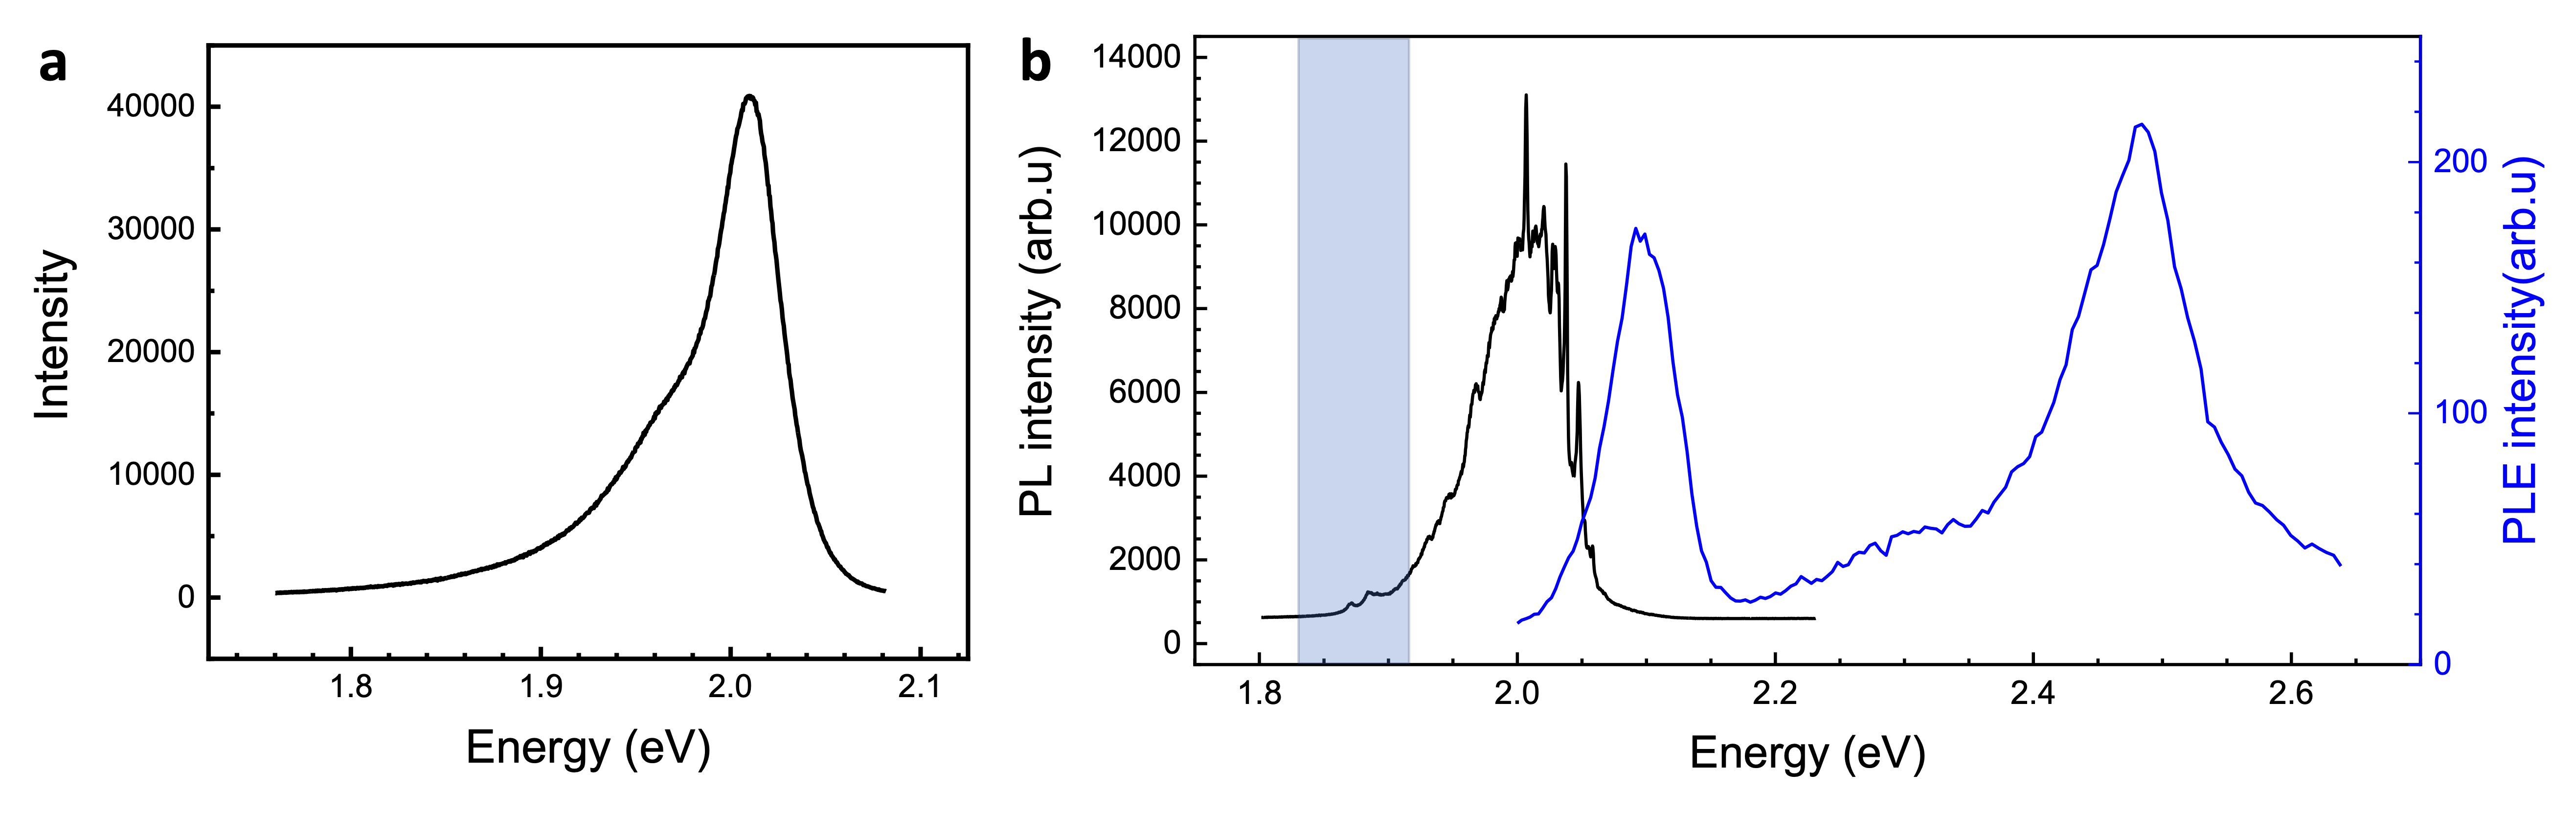
\includegraphics[width=\textwidth]{Figure/Chapter_four/pl_ple_nonencp.png}
    \caption{(a) PL spectrum of non-encapsulated WS$_2$ measured at room temperature (excitation: 473~nm, 1~$\mu$W). (b) PL spectrum (black) acquired at 3~K and corresponding PLE spectrum recorded over the spectral range indicated by the blue shaded region.}
    \label{fig:pl_ple_nonencp}
\end{figure}

Fig.~\ref{fig:pl_nonencp_annealing}(a) shows the evolution of the low-temperature photoluminescence spectrum of a non-encapsulated WS$_2$ monolayer as a function of annealing temperature. All spectra were acquired at $T_{\mathrm{meas}} = 30$~K after the sample had been annealed at the indicated temperature for 30~minutes and subsequently cooled to the measurement temperature, following the standardized protocol described in Section~\ref{subsec:Standardized Annealing Protocol}. The excitation source was a continuous-wave laser at $\lambda = 570$~nm with a power of $P = 5$~$\mu$W.

At room temperature and after mild annealing up to $\sim$600~K, the PL spectrum displays the broad excitonic emission of monolayer WS$_2$ centered around 2.0~eV, with no clearly resolved spectral features due to disorder broadening in the non-encapsulated configuration. No qualitative change in the PL spectrum is observed up to $\sim$800~K.

However, a qualitative change first appears after annealing at approximately 900--1000~K. A new emission feature develops on the low-energy side of the spectrum, initially as a broad shoulder and progressively gaining intensity as the annealing temperature is increased beyond 1000~K. By 1100--1200~K, this feature, which we label $X_L$ (localized emission), stands out as a distinct peak clearly separated from the main excitonic emission.

The $X_L$ peak is located approximately 220~meV below the neutral exciton energy $X_A^0$ at low temperature, placing it at approximately 1.82--1.84~eV. The emergence of this peak after high-temperature annealing suggests the formation of thermally induced defect states in the WS$_2$ lattice. The energy offset of $\sim$220~meV is comparable to the $\sim$200~meV offset reported for a spectrally narrow emission attributed to excitons localized at sulfur vacancies in monolayer MoS$_2$ \cite{mitterreiter2021role}, supporting a similar microscopic origin. In the MoS$_2$ system, this defect emission becomes visible after annealing at around 500~K and disappears above $\sim$900~K \cite{mitterreiter2021role}; in our WS$_2$ samples, the analogous emission requires higher annealing temperatures (above $\sim$1000~K), indicating a higher thermal threshold for the defect formation process in WS$_2$.

After annealing at 1200~K, $X_L$ reaches its maximum intensity relative to the neutral exciton. Fig.~\ref{fig:pl_nonencp_annealing}(b) shows the $X_L$ peak in detail at this annealing temperature: the emission is centered at approximately 1.84~eV and exhibits a Lorentzian lineshape with a full width at half maximum (FWHM) of $\sim$12~meV. While this linewidth is narrow compared to the broad excitonic emission of non-encapsulated samples at room temperature, it remains significantly 
broadened by inhomogeneous contributions arising from local disorder in 
the non-encapsulated configuration.

\begin{figure}[htbp]
    \centering
    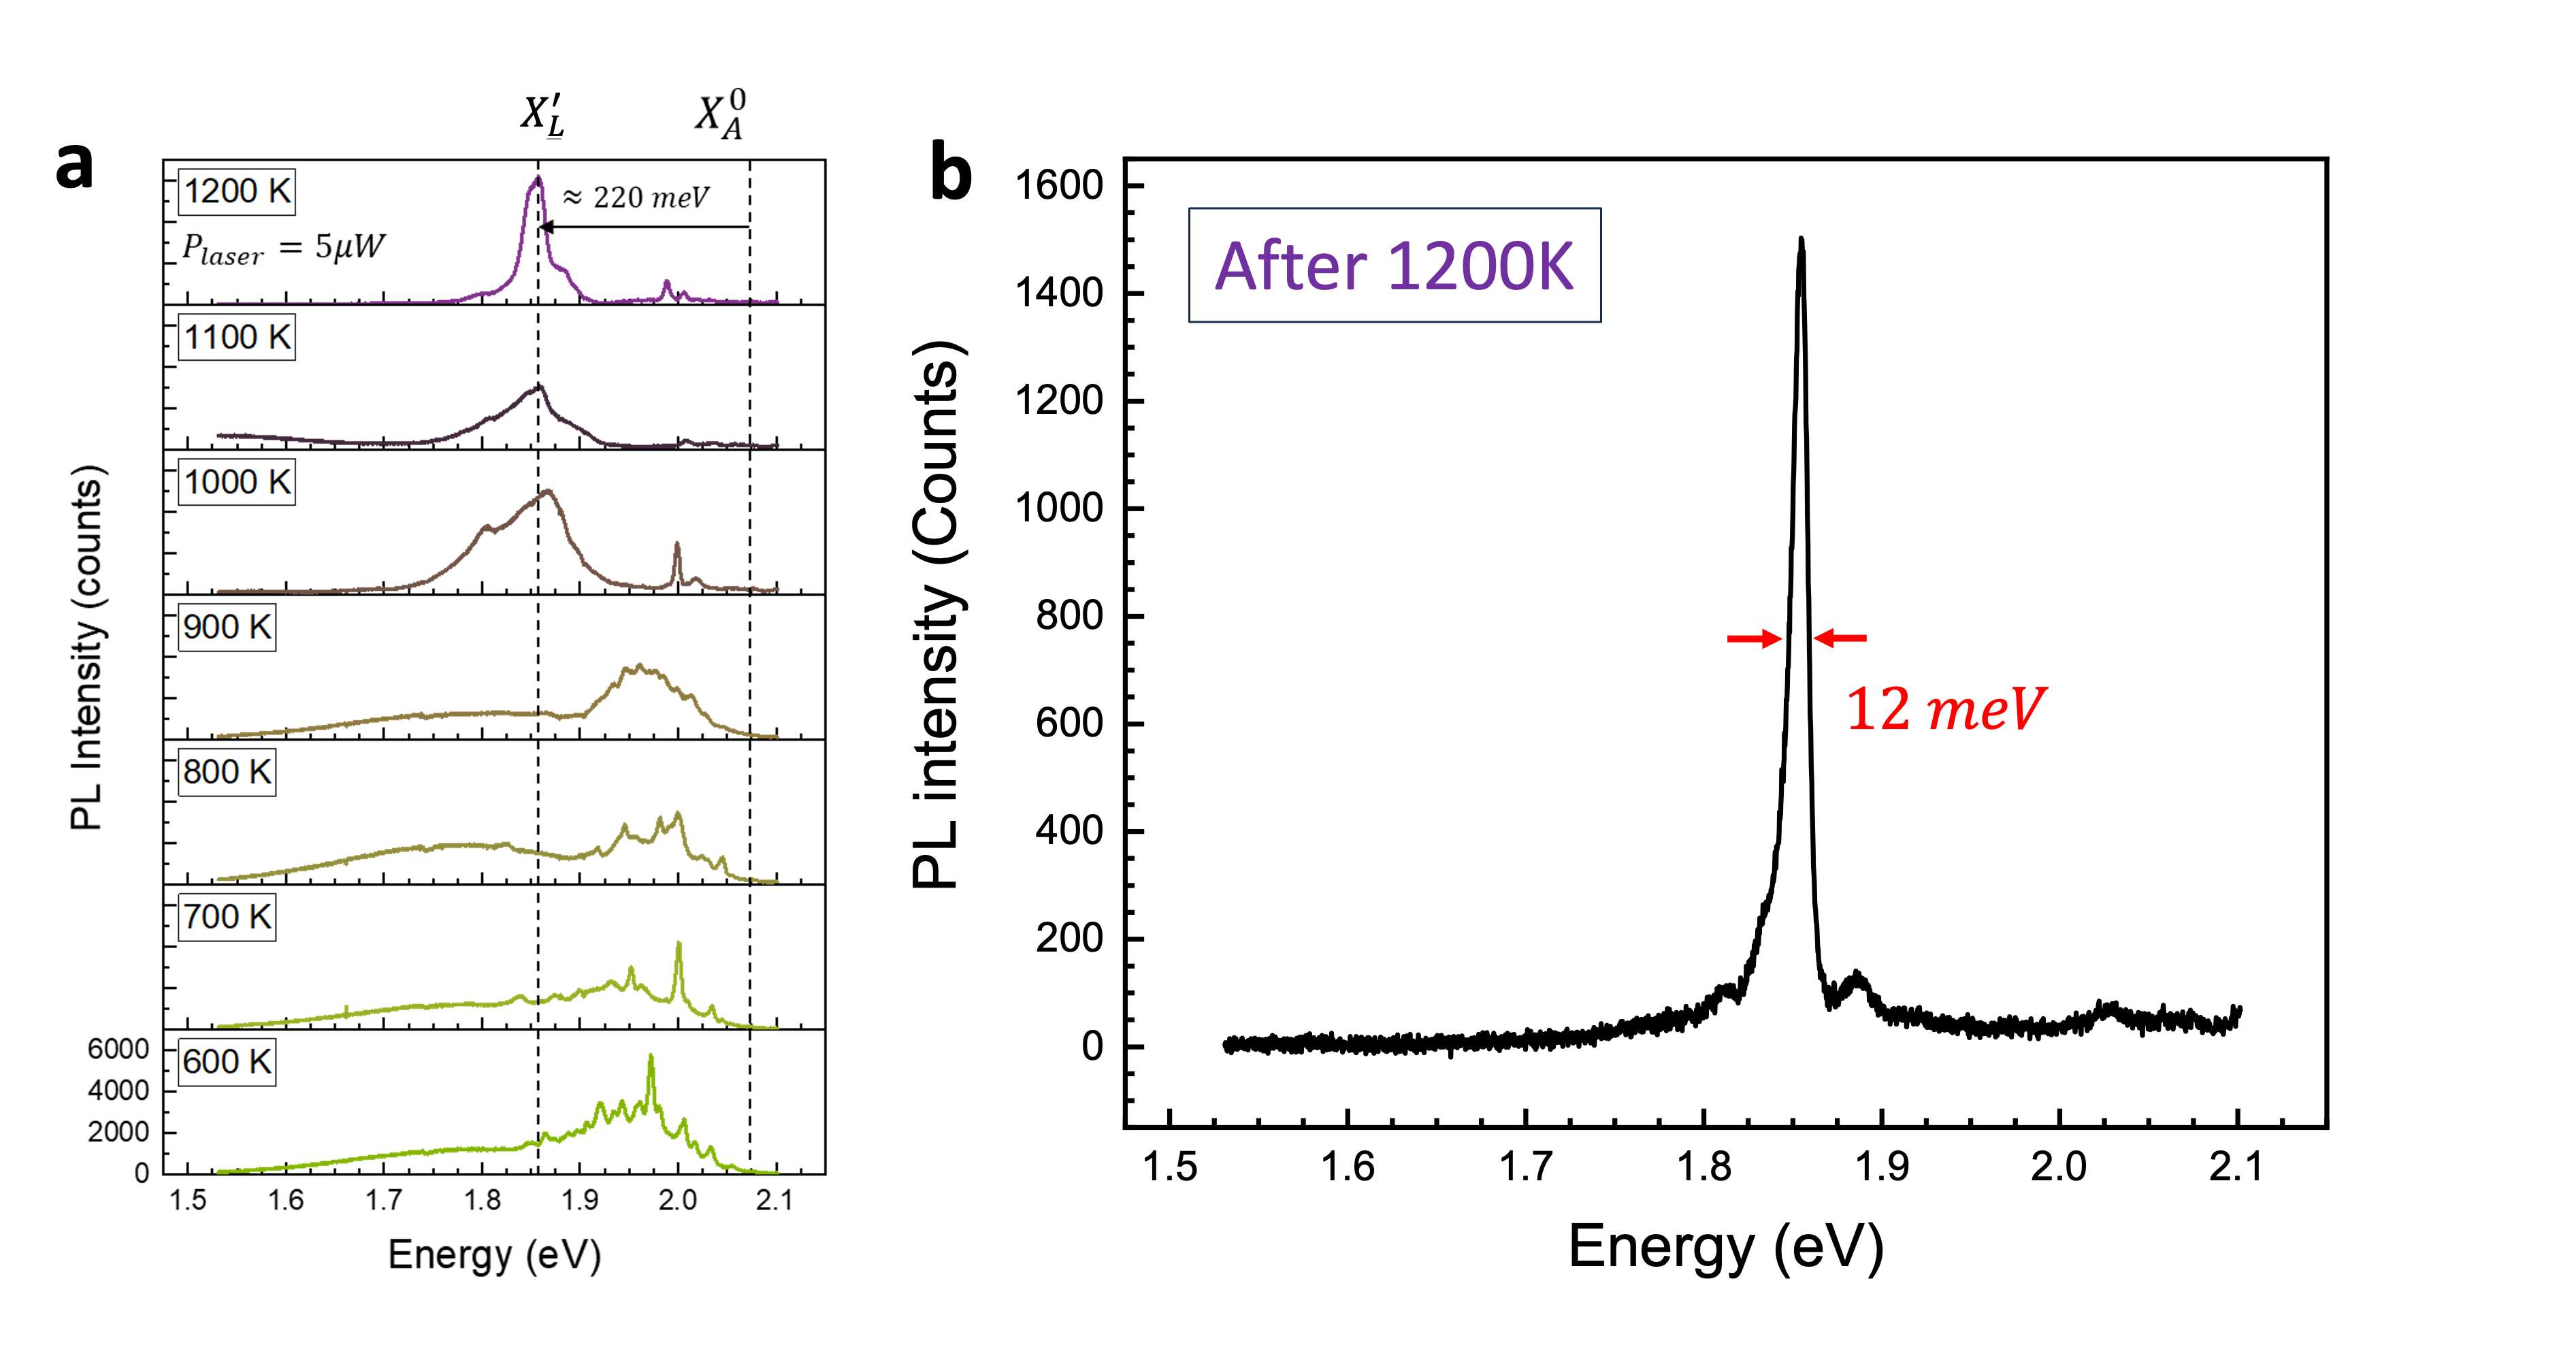
\includegraphics[width=\textwidth]{Figure/Chapter_four/pl_nonencp_annealing.png}
    \caption{(a) Evolution of the low-temperature ($T = 30$~K) PL spectrum of a non-encapsulated WS$_2$ monolayer after successive annealing steps from 600~K to 1200~K ($\lambda_{\mathrm{laser}} = 570$~nm, $P = 5$~$\mu$W). The $X_L$ peak emerges as a distinct feature above $\sim$1000~K and intensifies with increasing annealing temperature. Dashed lines indicate the positions of $X_L$ and $X_A^0$, separated by $\sim$220~meV. (b) Detailed spectrum of the $X_L$ emission after 1200~K annealing, showing a Lorentzian lineshape with FWHM $\approx 12$~meV.}
    \label{fig:pl_nonencp_annealing}
\end{figure}

\subsection{Power Dependence and Saturation Behavior}
\label{subsec:Power Dependence and Saturation Behavior}

To gain insight into the nature of the $X_L$ emission---specifically, whether it arises from a finite ensemble of defect states---we performed power-dependent PL measurements on the $X_L$ peak after annealing at 1200~K. Fig.~\ref{fig:power_dep_nonencp} shows the peak intensity of $X_L$ as a function of laser power on a double-logarithmic scale, measured at $T = 30$~K.

At low excitation powers, the $X_L$ intensity grows with laser power with a log--log slope of approximately 0.74, approaching linear behavior. As the power increases above $\sim$1~$\mu$W, the emission intensity progressively approaches saturation, reaching a plateau near $\sim$6~$\mu$W. This saturation behavior is consistent with a finite number of optically active defect states: once the accessible emitters are driven to their excited state, additional excitation cannot further increase the emission rate.

\begin{figure}[htbp]
    \centering
    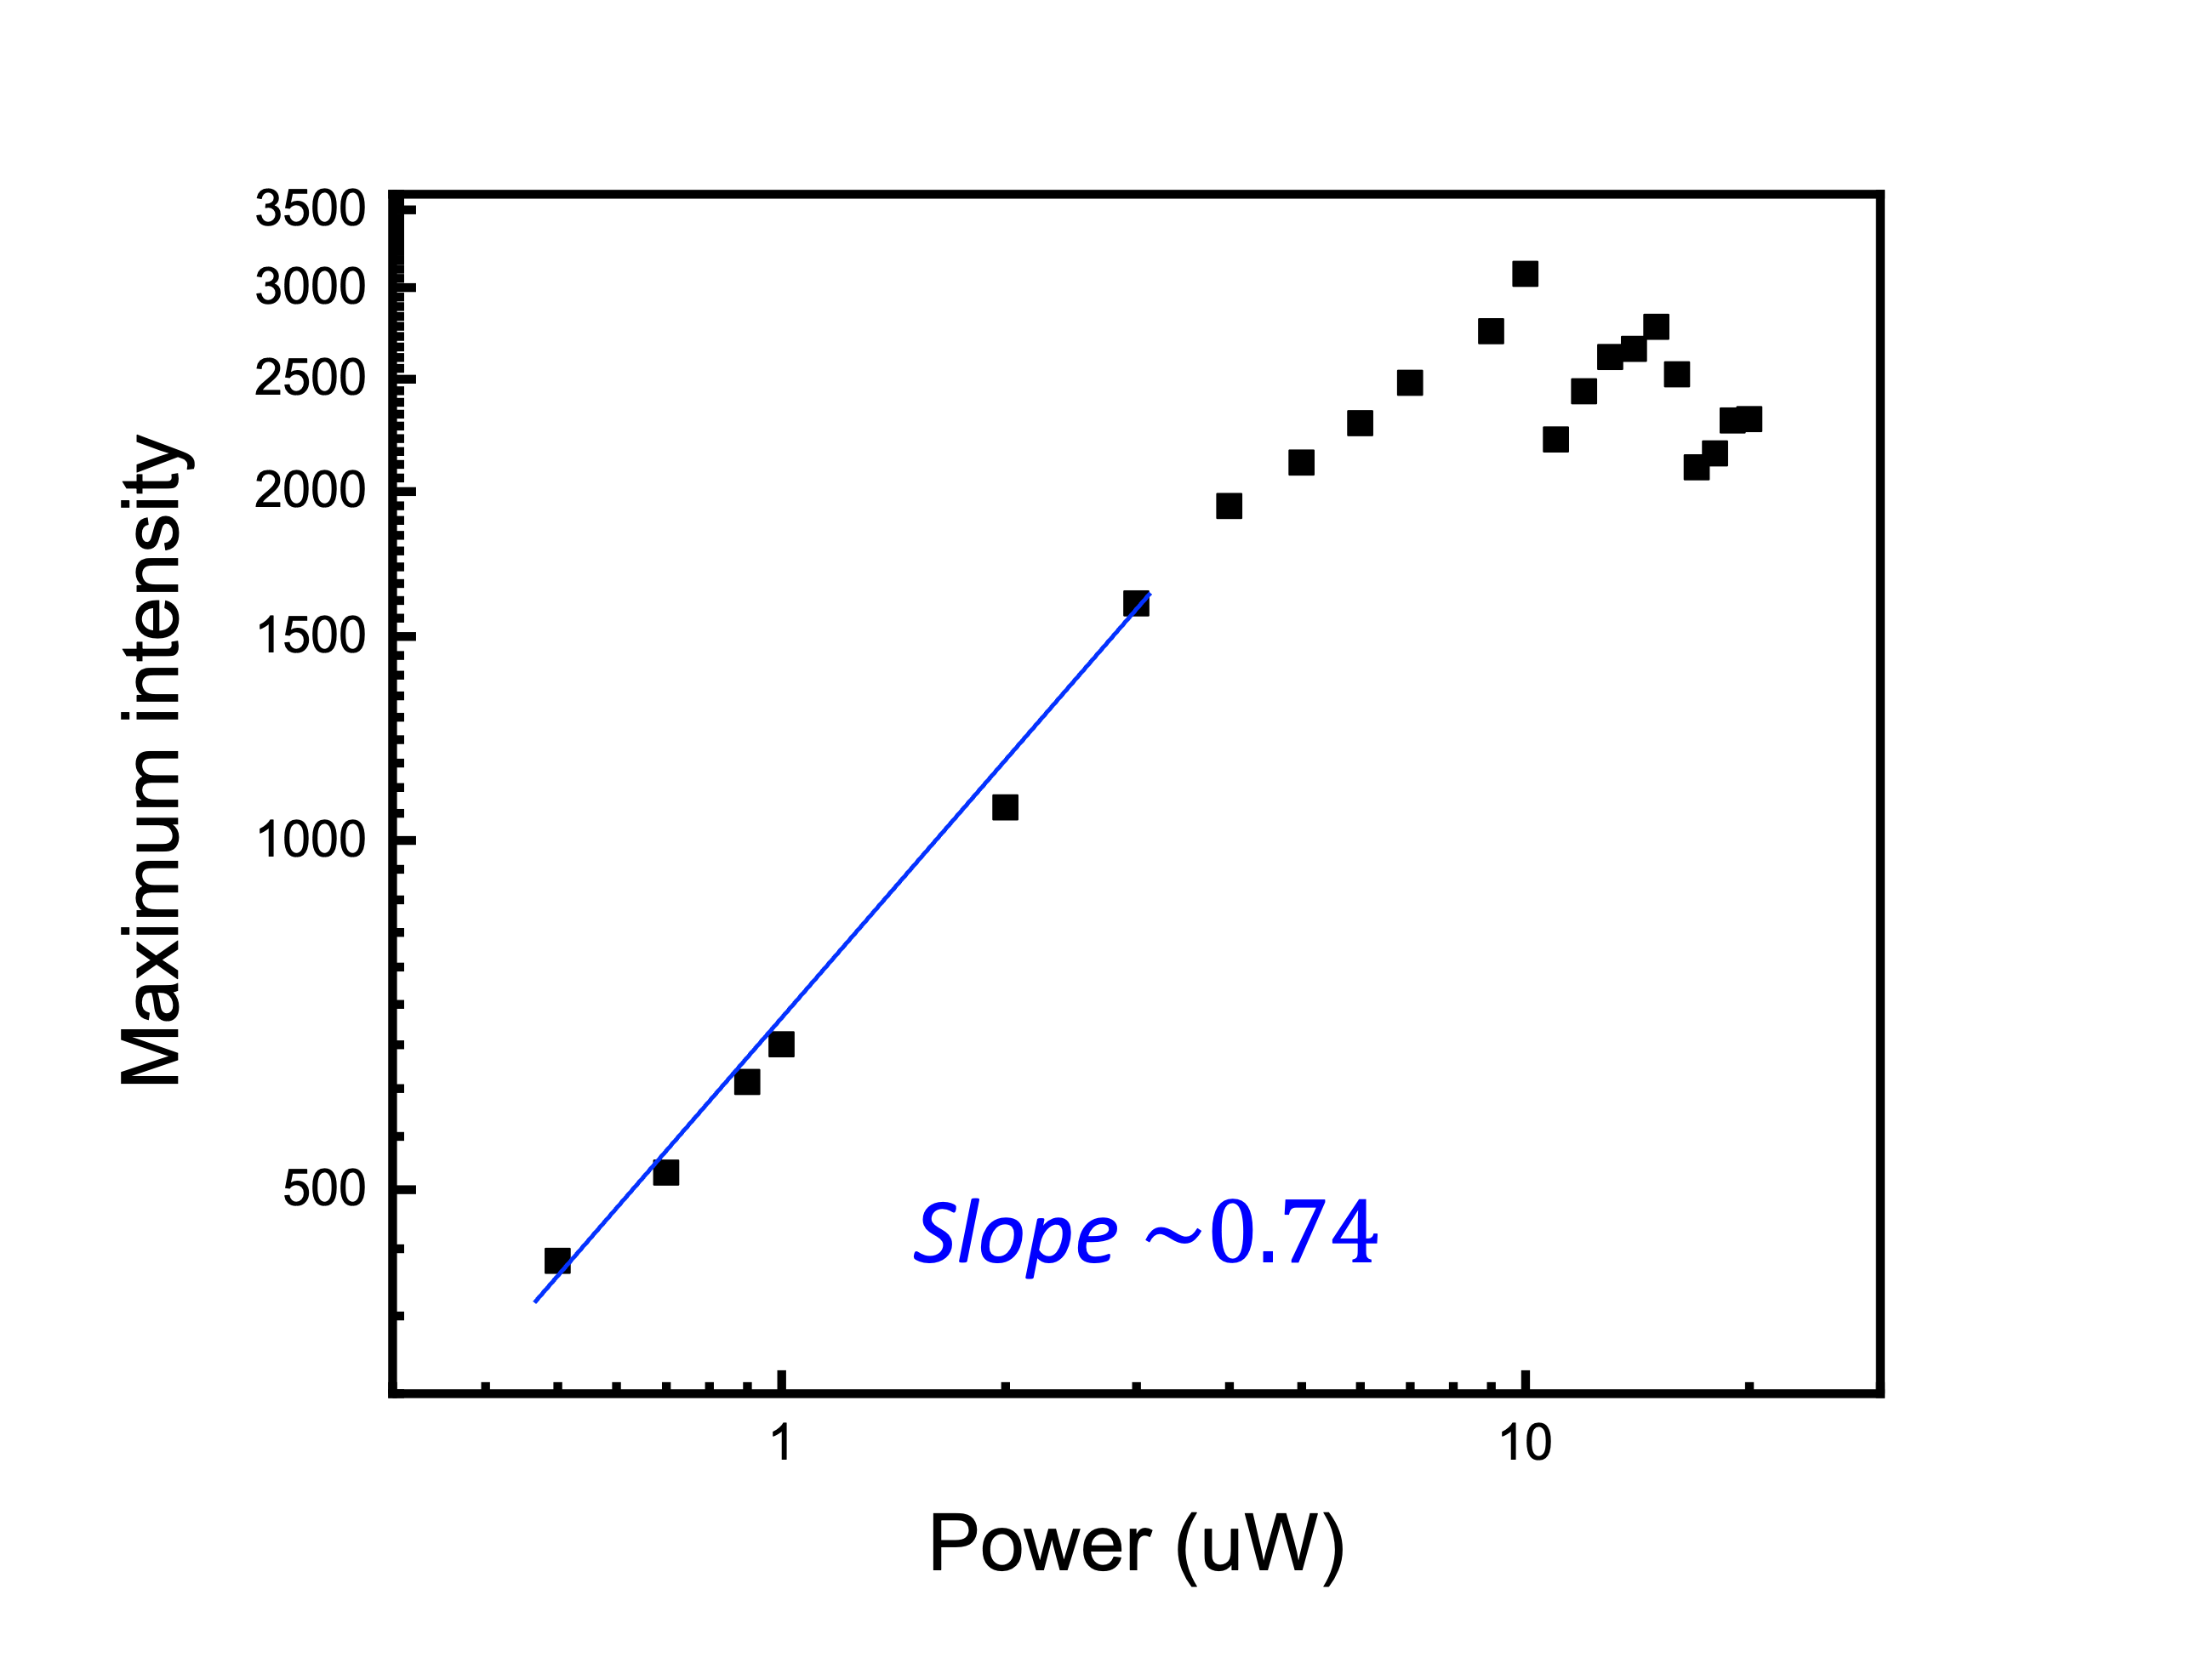
\includegraphics[width=0.6\textwidth]{Figure/Chapter_four/power_dep_nonencp.png}
    \caption{Power dependence of the $X_L$ emission intensity in a non-encapsulated WS$_2$ monolayer after 1200~K annealing, measured at $T = 30$~K under CW excitation ($\lambda = 570$~nm). The log--log plot reveals a sub-linear regime at low power (slope $\approx 0.74$, dashed line) followed by saturation above $\sim$6~$\mu$W, consistent with a finite density of defect emitters.}
    \label{fig:power_dep_nonencp}
\end{figure}

\subsection{Temperature Dependence of the $X_L$ Intensity}
\label{subsec:Temperature Dependence of the $X_L$ Intensity}

Having established that $X_L$ saturates at a finite power level characteristic of localized emitters, we now examine its behavior as a function of the measurement temperature. This is distinct from the annealing temperature discussed above: here, the annealing is fixed at 1200~K to maximize $X_L$ intensity, and the cryostat temperature $T_{\mathrm{meas}}$ is varied using the built-in heater, while keeping the chip heater current at zero.

Fig.~\ref{fig:temp_dep_xl_nonencp} shows the PL spectra recorded at measurement temperatures from 27~K to 100~K, along with the integrated $X_L$ intensity as a function of temperature. The emission is visible and relatively intense from 27~K to approximately 35--40~K, where it reaches a maximum. Above 40~K, the $X_L$ intensity decreases rapidly and becomes undetectable by $\sim$100~K. This thermal quenching defines an upper operating temperature for $X_L$ in non-encapsulated WS$_2$, severely limiting its practical utility.

The rapid quenching of $X_L$ above $\sim$40~K, with complete disappearance by $\sim$100~K, indicates a relatively shallow localization energy of the defect state in the non-encapsulated configuration. This limited operating temperature range is one of the fundamental challenges for defect emitters in non-encapsulated samples.

\begin{figure}[htbp]
    \centering
    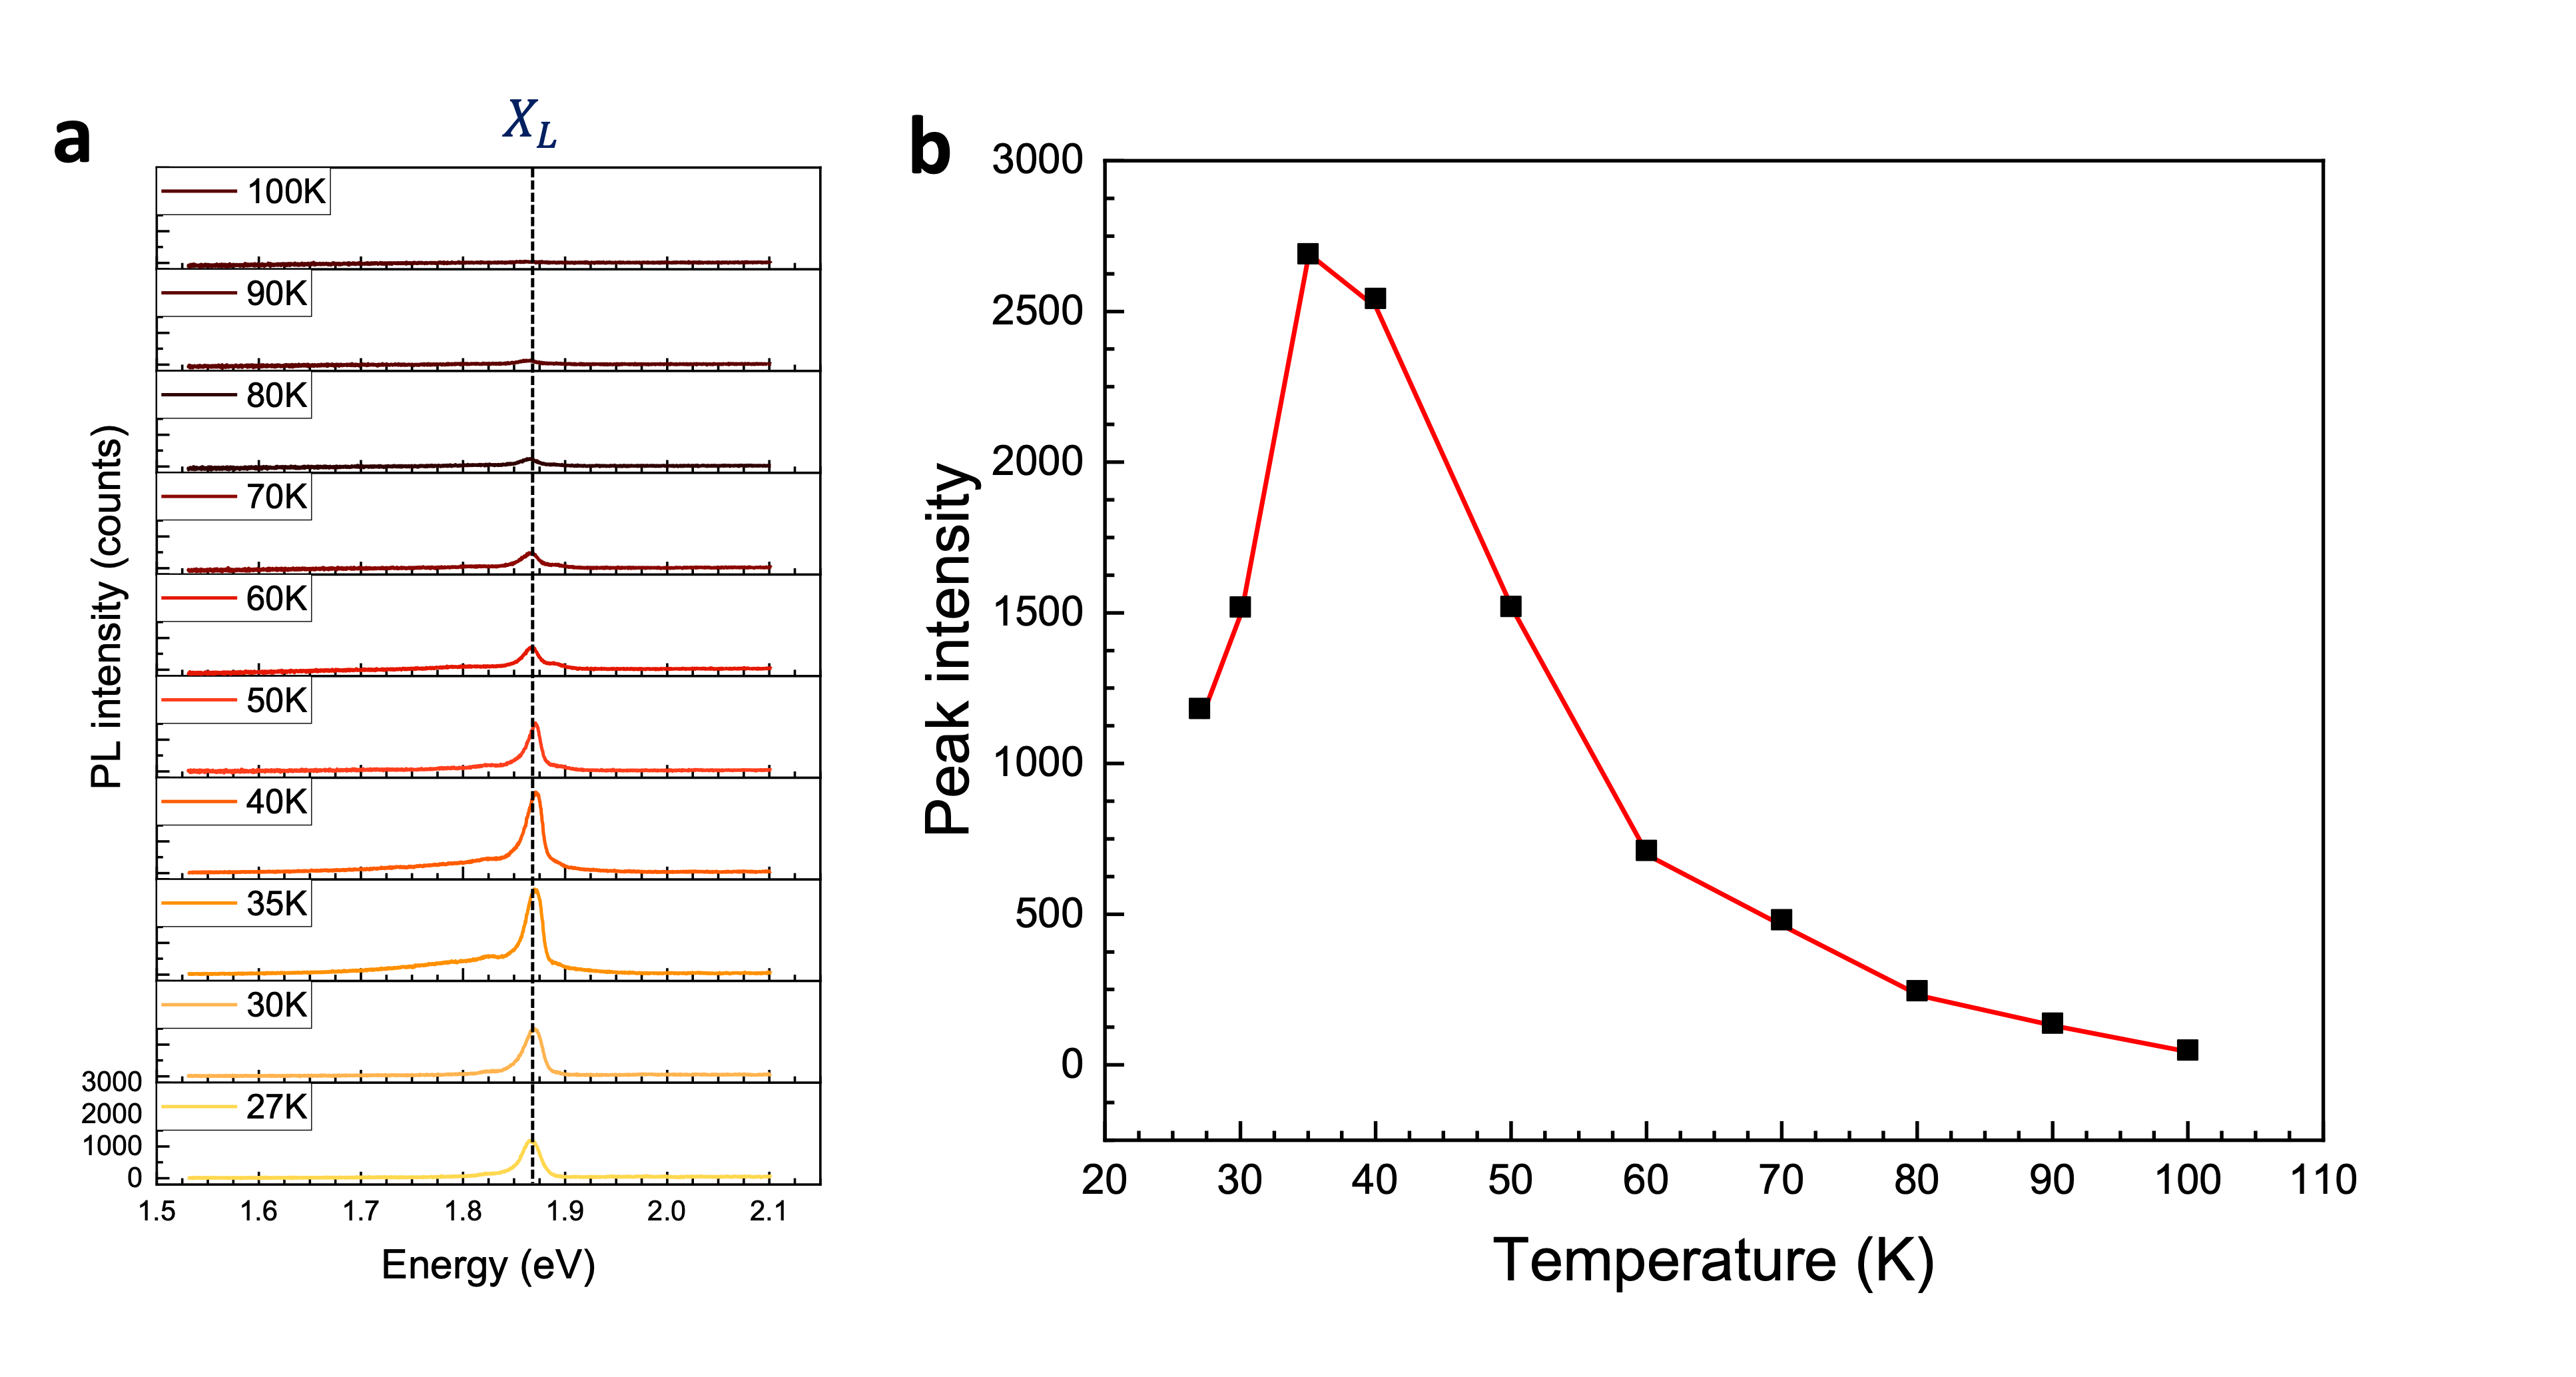
\includegraphics[width=\textwidth]{Figure/Chapter_four/temp_dep_xl_nonencp.png}
    \caption{(a) PL spectra of $X_L$ in a non-encapsulated WS$_2$ monolayer (after 1200~K annealing) at measurement temperatures from 27~K to 100~K. (b) Integrated $X_L$ intensity as a function of measurement temperature, showing a maximum near 35~K and complete quenching above $\sim$100~K.}
    \label{fig:temp_dep_xl_nonencp}
\end{figure}



\subsection{Optical Limitations and the Necessity of Encapsulation}
\label{subsec:Optical Limitations and the Necessity of Encapsulation}

Despite providing experimental evidence for thermally activated defect emission in WS$_2$, the non-encapsulated configuration suffers from several fundamental limitations that hinder both rigorous spectroscopic analysis and quantum optical characterization.


\textbf{Spectral clarity and reference exciton peaks.} A key limitation of non-encapsulated WS$_2$ is the complexity of its low-temperature PL spectrum: the emission is dominated by a large number of unresolved excitonic complexes whose microscopic origin cannot be unambiguously identified, and the neutral exciton $X_A^0$ is not clearly observable as a distinct peak. This spectral congestion prevents a precise determination of the energy reference from which newly emerging features can be characterized.

In contrast, hBN-encapsulated WS$_2$ monolayers exhibit a markedly improved spectral quality at low temperature. The spectrum resolves into a set of well-defined peaks with stable energetic positions that serve as reliable spectral references \cite{zinkiewicz-2021c}. This allows any annealing-induced emission feature to be characterized precisely in terms of its energy offset relative to the known excitonic transitions, enabling a more rigorous physical analysis than is possible in the non-encapsulated case.

\textbf{Broad linewidth.} The $X_L$ linewidth of $\sim$12~meV is significantly broader than the few-meV linewidths typically observed for excitonic emissions in hBN-encapsulated WS$_2$ monolayers at low temperature~\cite{cadiz-2017}, indicating that the $X_L$ emission remains inhomogeneously broadened in the non-encapsulated configuration. This excess broadening originates from dielectric disorder: fluctuations of the local electrostatic environment at the exposed WS$_2$ surface induce a distribution of emission energies across individual defect sites~\cite{raja-2019}.

\textbf{Photo-doping instability.} A particularly problematic artifact in non-encapsulated TMD samples is photo-doping: laser illumination generates free carriers that become trapped at defect states in the SiO$_2$ substrate and subsequently transferred to the TMD monolayer, modifying the local doping level and thereby the exciton emission properties. Strikingly, this effect occurs even at excitation powers as low as 1~$\mu$W~$\mu$m$^{-2}$, commonly assumed to be non-intrusive: the trion-to-exciton PL ratio increases irreversibly, the total PL intensity decreases, and the neutral exciton emission can disappear entirely~\cite{cadiz-2016}. In practice, this manifests as a progressive shift of the PL peak position and a change in the relative weights of neutral and charged exciton emission during a single measurement, rendering quantitative spectroscopy unreliable. Furthermore, photon correlation measurements such as $g^{(2)}(\tau)$ require prolonged acquisition times to accumulate sufficient statistics. In non-encapsulated samples, the continuous drift of the emission energy induced by photo-doping prevents stable long-duration measurements, making it impractical to characterize the quantum optical nature of $X_L$ in this configuration.

\textbf{High activation temperature.} The onset of $X_L$ emission above $\sim$1000~K in non-encapsulated WS$_2$ is close to the thermal dissociation threshold of the monolayer ($\sim$1000--1273~K, as established by Raman spectroscopy in Chapter~\ref{chap:three}). This leaves only a narrow temperature window in which defect emission can be generated without simultaneously destroying the sample. hBN encapsulation is therefore expected to play a stabilizing role during high-temperature annealing.

These limitations collectively motivate the transition to hBN-encapsulated WS$_2$ monolayers, which is the focus of the remainder of this chapter and of Chapter~\ref{chap:five}.



\section{Optical Baseline of hBN-Encapsulated WS$_2$} % (fold)
\label{sec:Optical Baseline of hBN-Encapsulated WS$_2$}

The fabrication of hBN/WS$_2$/hBN heterostructures and their transfer onto SiC micro-heater chips was described in Chapter~\ref{chap:methodology}. Before thermal annealing is applied, it is essential to establish the optical baseline of the pristine encapsulated sample at cryogenic temperature. This baseline serves as a reference against which any annealing-induced modifications can be unambiguously identified, and also demonstrates the superior optical quality that encapsulation provides.

\subsection{Low-Temperature PL Spectrum: Excitonic Complexes in Pristine Samples}
\label{subsec:Low-Temperature PL Spectrum}

Fig.~\ref{fig:pl_encp_pristine} shows the PL spectrum of a pristine hBN-encapsulated WS$_2$ monolayer at $T = 3.66$~K, measured with a continuous-wave 514.5~nm laser at $P = 1$~$\mu$W. The spectrum displays a remarkably rich and well-resolved set of narrow excitonic peaks, a direct consequence of the atomically flat and chemically inert dielectric environment provided by the hBN cladding layers, attesting to the excellent optical quality of the encapsulated sample.

\begin{figure}[htbp]
    \centering
    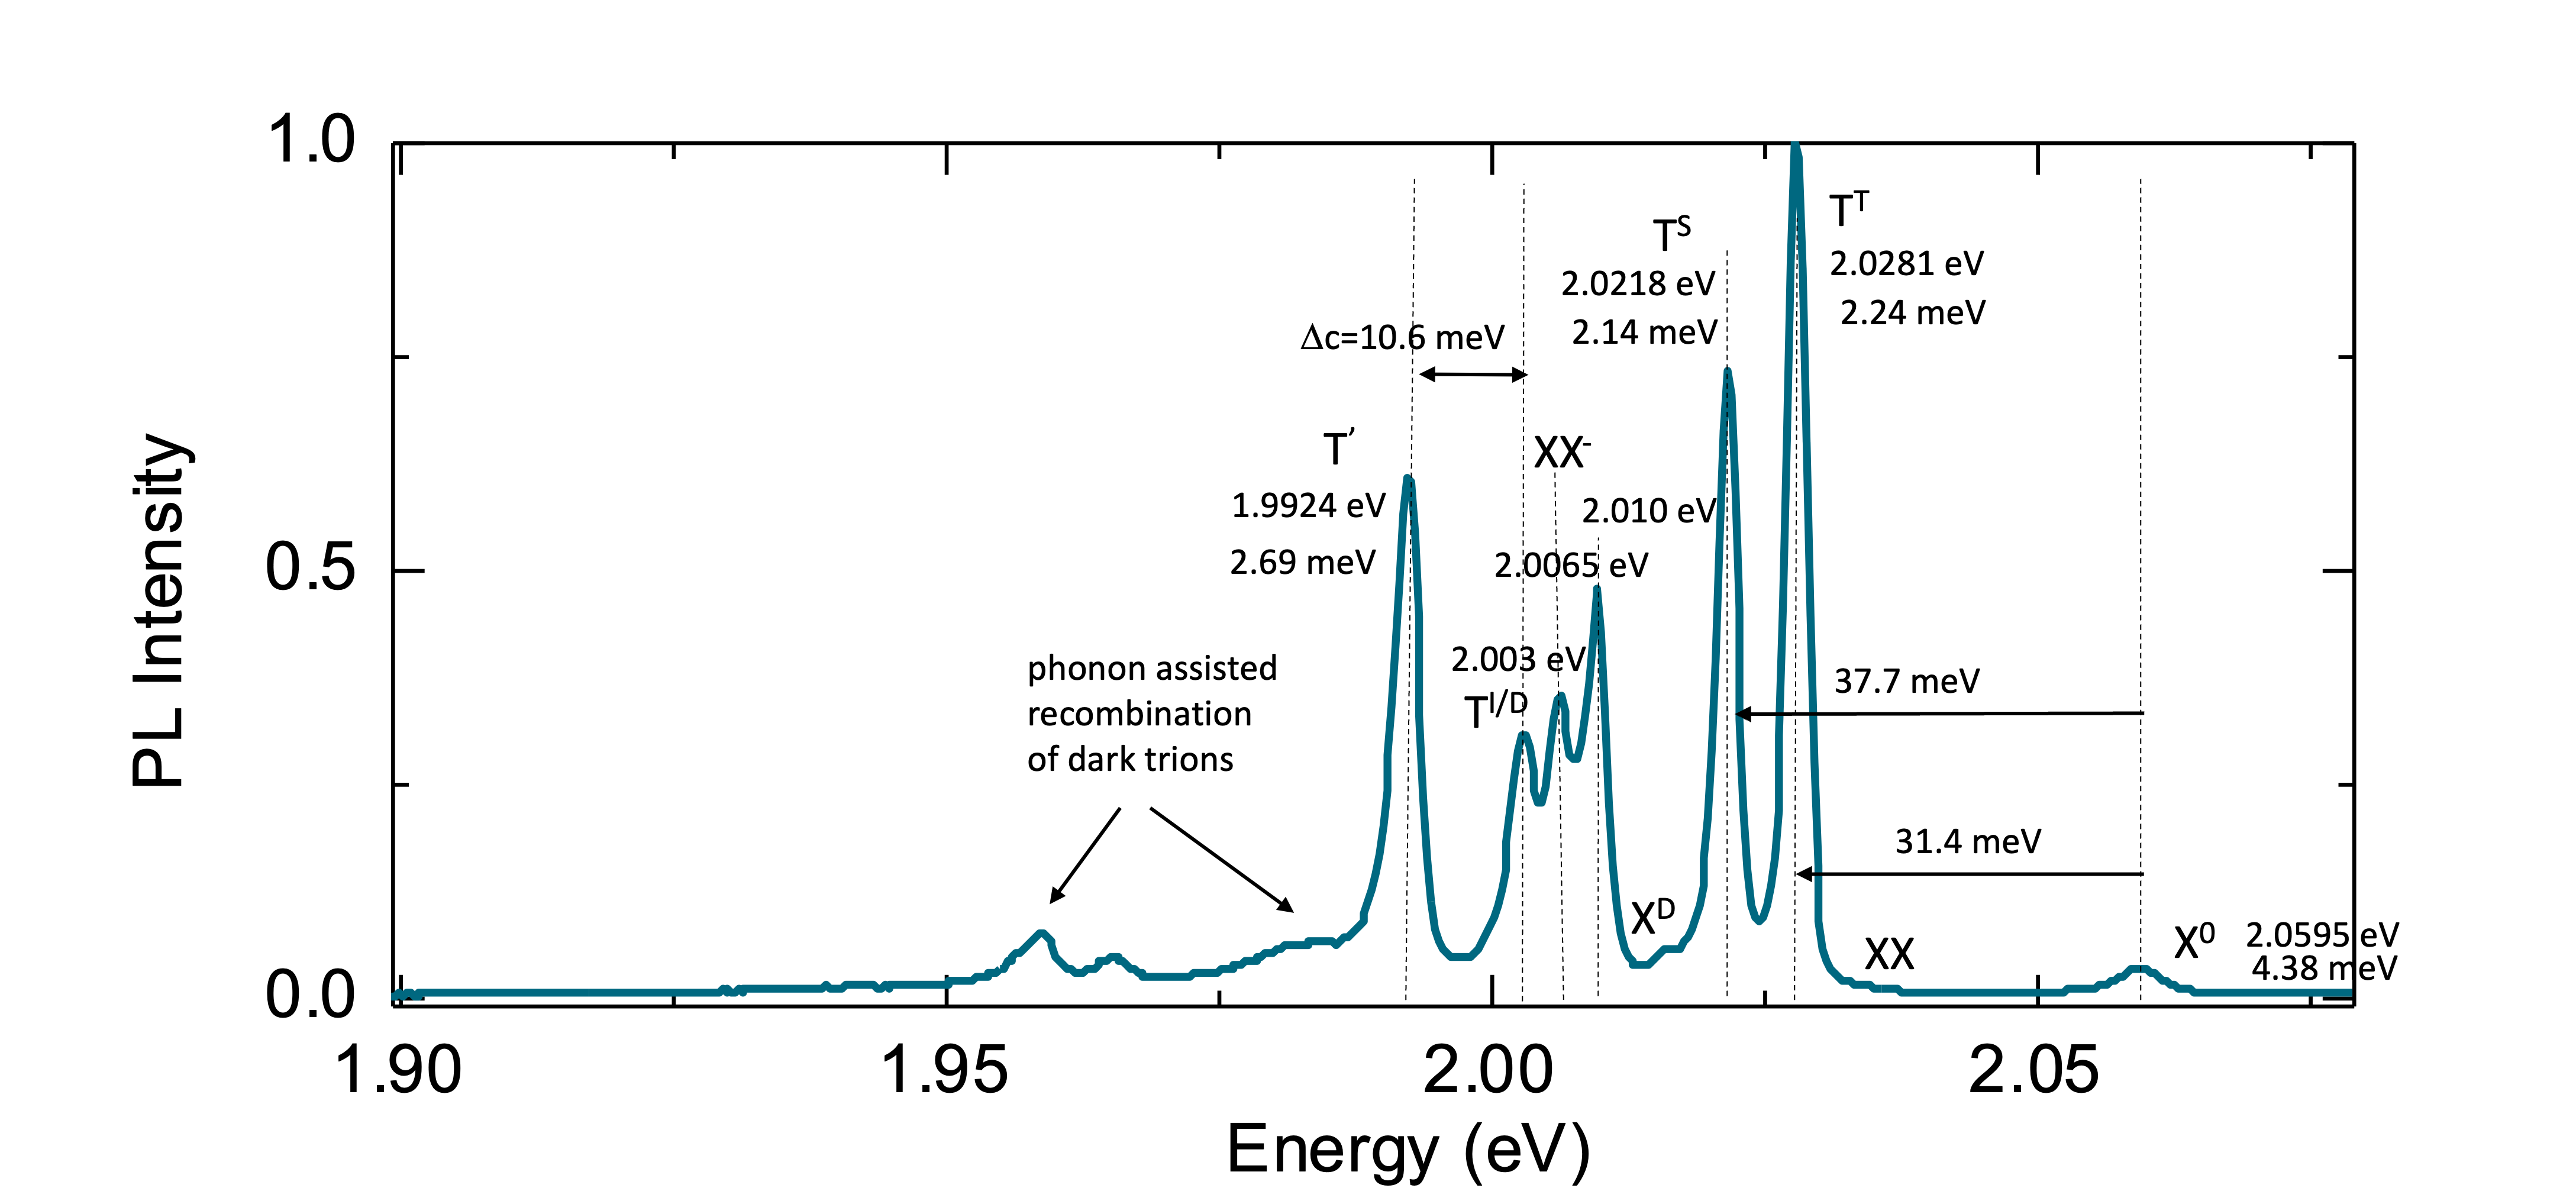
\includegraphics[width=\textwidth]{Figure/Chapter_four/pl_encp_pristine.png}
    \caption{PL spectrum of a pristine hBN-encapsulated WS$_2$ monolayer at $T = 3.66$~K ($\lambda_{\mathrm{laser}} = 514.5$~nm, $P = 1$~$\mu$W), showing the neutral exciton $X_A^0$, intervalley triplet trion $T^T$, intravalley singlet trion $T^S$, negative biexciton $XX^-$, intervalley dark trion $T^I$, semidark trion $T'$, and phonon-assisted dark trion replicas. All peaks are labeled with their assigned identities.}
    \label{fig:pl_encp_pristine}
\end{figure}

The dominant feature at high energy is the neutral exciton $X_A^0$, located at approximately 2.060~eV with a linewidth of $\sim$4.4~meV. This linewidth, while reflecting both homogeneous and residual inhomogeneous broadening, is already far narrower than the $\sim$20--50~meV widths typical of TMDs on SiO$_2$ substrates~\cite{cadiz-2017}. The encapsulation suppresses the dominant sources of disorder---surface roughness, trapped charges, and polar phonon modes of the substrate---yielding an optical quality comparable to state-of-the-art encapsulated TMD samples~\cite{raja-2017}.

Below $X_A^0$, the spectrum displays a series of negatively charged excitonic complexes. In tungsten-based darkish monolayers such as WS$_2$, there are four distinct negative trions---two bright and two dark---arising from the possible spin and valley configurations of the two electrons forming the trion. The two bright (optically active) trions are the intravalley singlet $T^S$ and the intervalley triplet $T^T$, in which both electrons reside in the same valley or in opposite valleys, respectively. The two dark (optically inactive) trions are the intravalley spin-forbidden $T^D$ and the intervalley momentum-forbidden $T^I$, which cannot recombine directly due to spin and momentum conservation rules. Among these, $T^D$ is not directly observable at zero magnetic field. These four configurations are schematically illustrated in Fig.~\ref{fig:negative_trions}~\cite{zinkiewicz-2021c}.

\begin{figure}[htbp]
    \centering
    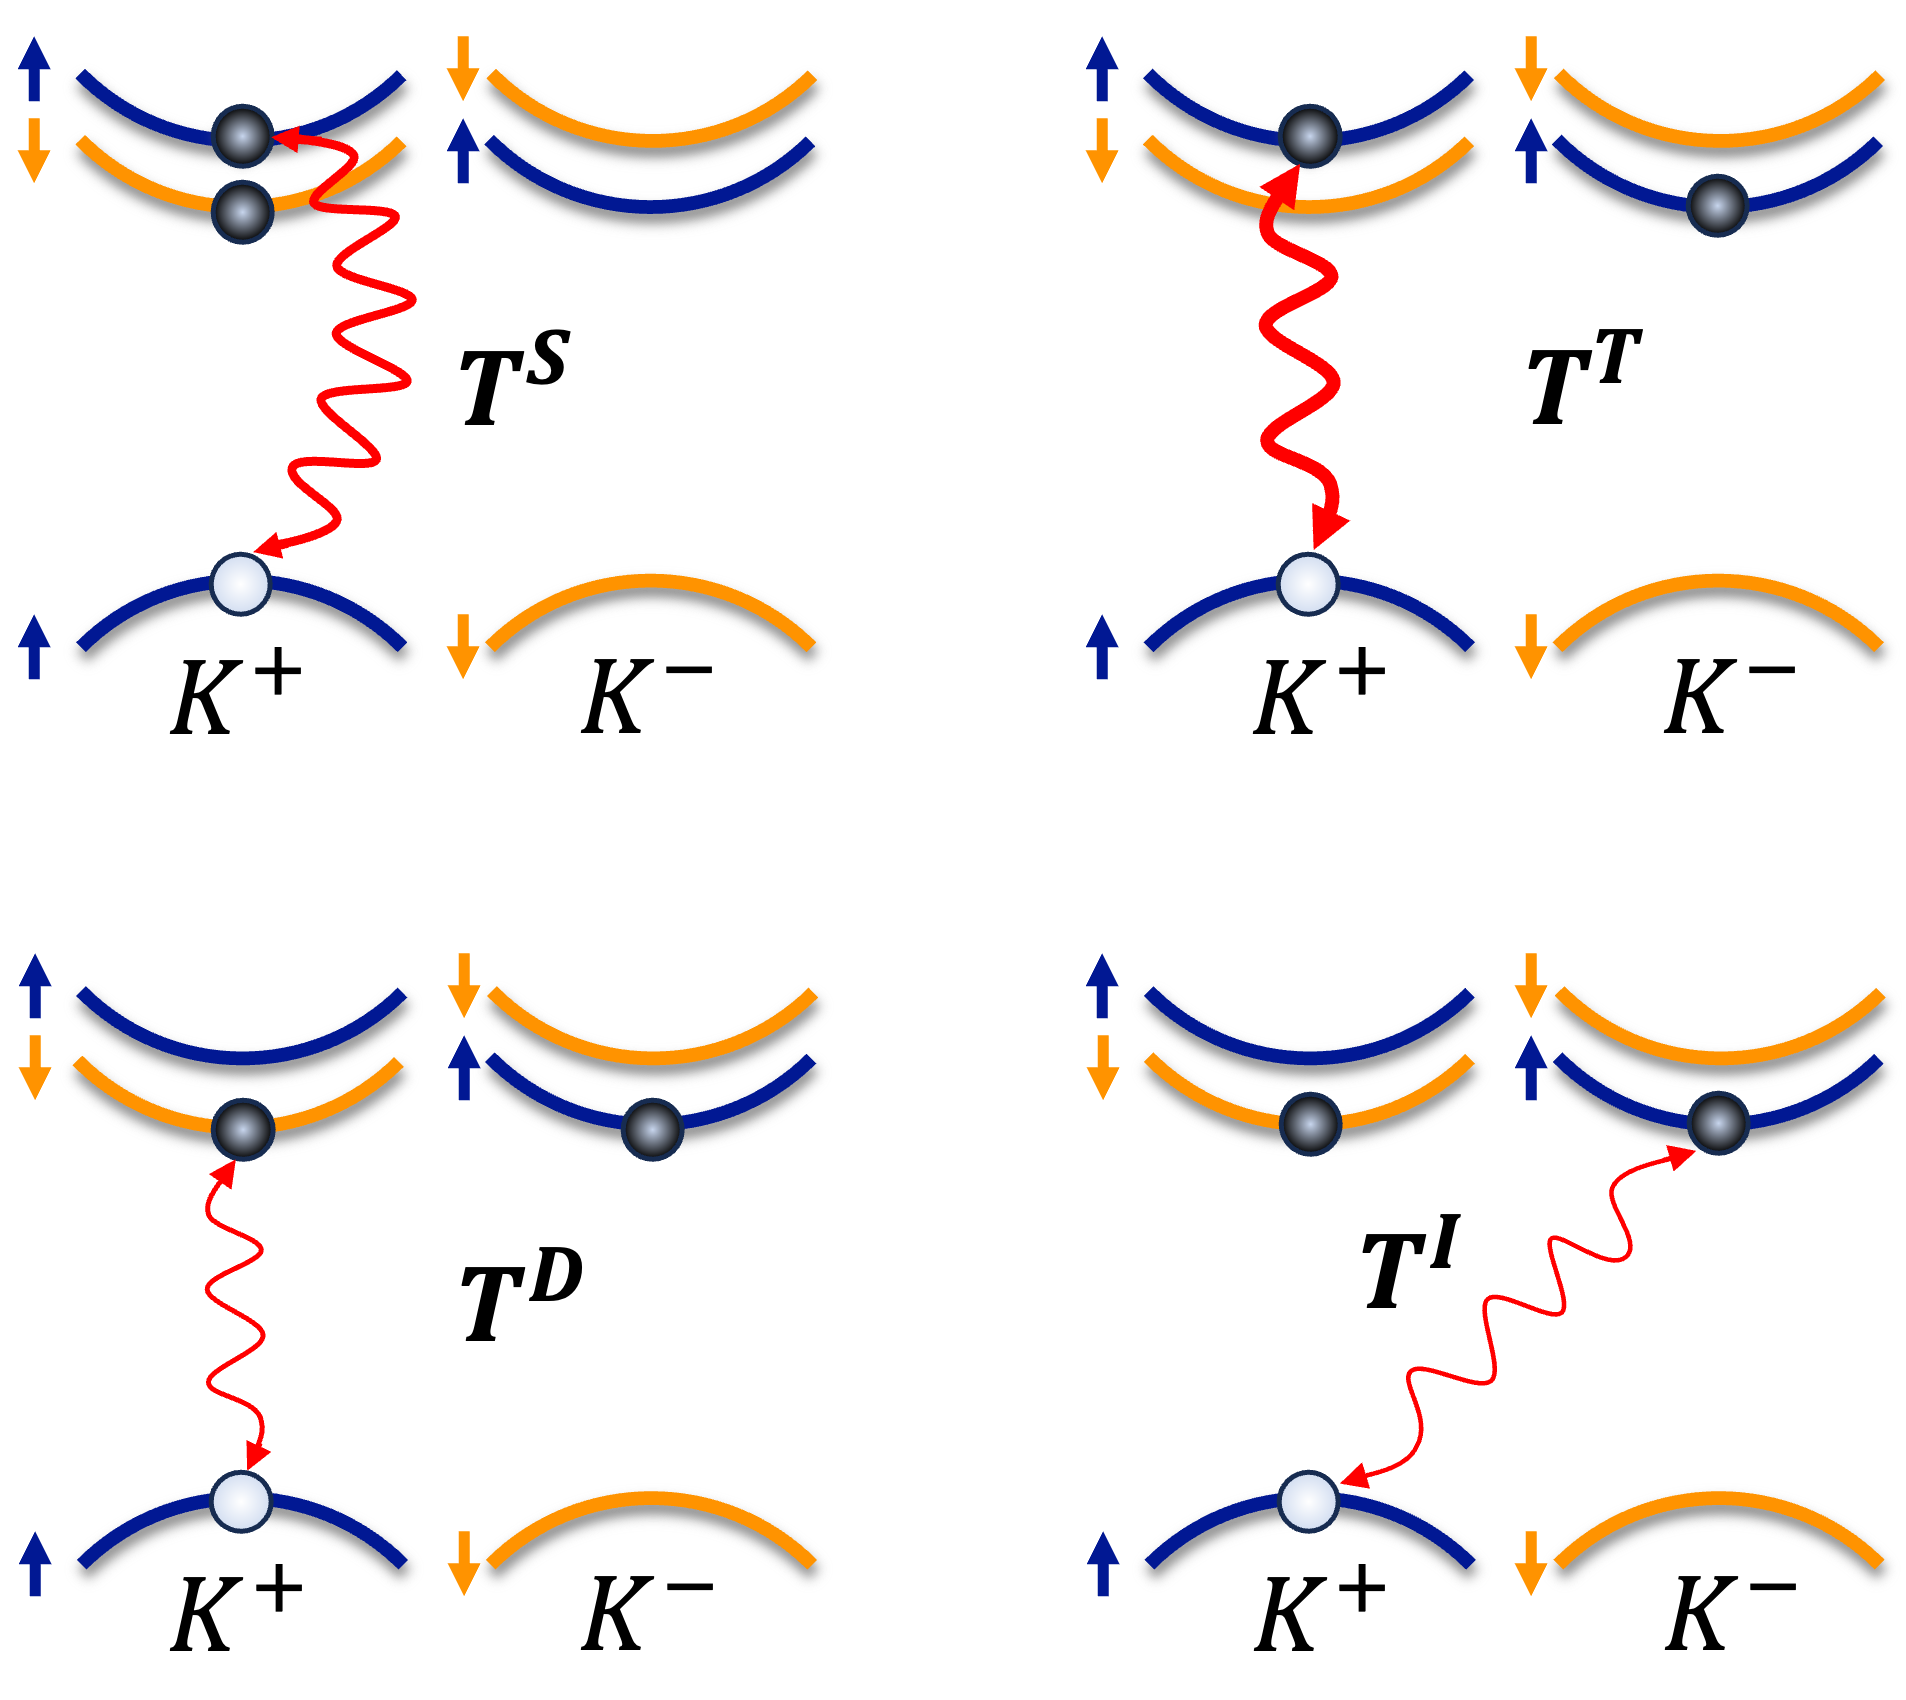
\includegraphics[width=0.6\textwidth]{Figure/Chapter_four/negative_trions.png}
    \caption{Schematic illustration of possible spin configurations for negatively charged excitons in WS$_2$ monolayer. $T^S$ and $T^T$ correspond to the bright intravalley singlet and intervalley triplet trions, whereas $T^D$ and $T^I$ represent the dark intravalley spin-forbidden and intervalley momentum-forbidden complexes, respectively. Adapted from~\cite{zinkiewicz-2021c}.}
    \label{fig:negative_trions}
\end{figure}

In the present spectrum, the bright trions $T^T$ and $T^S$ are resolved at $\sim$2.028~eV (linewidth $\sim$2.2~meV) and $\sim$2.022~eV (linewidth $\sim$2.1~meV), corresponding to binding energies of $\sim$32~meV and $\sim$38~meV relative to $X_A^0$, respectively, with an energy splitting of $\sim$6~meV between the two states. At slightly lower energies, the negative biexciton $XX^-$ appears at $\sim$2.007~eV, a complex only resolvable in high-quality encapsulated samples with sufficiently narrow intrinsic linewidths. The intervalley momentum-forbidden dark trion $T^I$ is observed at $\sim$2.003~eV, which may be enabled by defect states providing momentum conservation during recombination~\cite{zinkiewicz-2021c}. A weak emission feature attributed to the neutral dark exciton $X^{D}$ is also visible in the spectrum, consistent with the partial optical activation of the spin-forbidden dark neutral exciton state in high-quality encapsulated samples~\cite{zinkiewicz-2020a}.

The peak $T'$ at $\sim$1.992~eV (linewidth $\sim$2.7~meV) is identified as the semidark trion: a dark trion rendered optically active through electron--electron (e--e) scattering, which transfers an electron from the lower conduction band subband at K$^\pm$ to the higher subband at the opposite K$^\mp$ valley, enabling radiative recombination of the resulting e--h pair~\cite{zinkiewicz-2021c}.

At the lowest energies of the spectrum, a series of peaks arising from phonon-assisted recombination of the dark trion $T^D$ are observed. These phonon replicas originate from recombination pathways in which zone-edge phonons from the K and $\Gamma$ points of the Brillouin zone provide the spin- or momentum-flip required for the otherwise optically inactive dark trion to recombine radiatively~\cite{zinkiewicz-2021c}. The resolution of these phonon-assisted features serves as a sensitive marker of sample quality, as they are only accessible in encapsulated samples with sufficiently narrow intrinsic linewidths.

\subsection{Polarization-Resolved PL}
\label{subsec:Polarization-Resolved PL}

To investigate the valley polarization properties of the excitonic features, we performed circularly polarized PL spectroscopy, as described in Chapter~\ref{chap:methodology}. Co-polarized spectra are acquired with matching excitation and detection helicities ($\sigma^+/\sigma^+$ or $\sigma^-/\sigma^-$), while cross-polarized spectra are acquired with opposite helicities ($\sigma^+/\sigma^-$ or $\sigma^-/\sigma^+$). The degree of circular polarization (DOCP) is defined as

\begin{equation}
    \text{DOCP} = \frac{I_{\sigma^+\sigma^+} - I_{\sigma^+\sigma^-}}{I_{\sigma^+\sigma^+} + I_{\sigma^+\sigma^-}}.
\end{equation}

Fig.~\ref{fig:pl_pol_encap} shows a representative circularly polarized PL spectrum. The co- and cross-polarized spectra are nearly identical across most of the spectral range, with the most notable contrast appearing in the trion region. The singlet trion $T^S$ exhibits the largest DOCP of approximately 20\%, while the triplet trion $T^T$ shows a smaller but non-negligible polarization of $\sim$10\%, consistent with their respective intravalley and intervalley spin configurations~\cite{zinkiewicz-2021c}. The remaining excitonic features, including the neutral exciton $X_A^0$, show negligible circular polarization.

\begin{figure}[htbp]
    \centering
    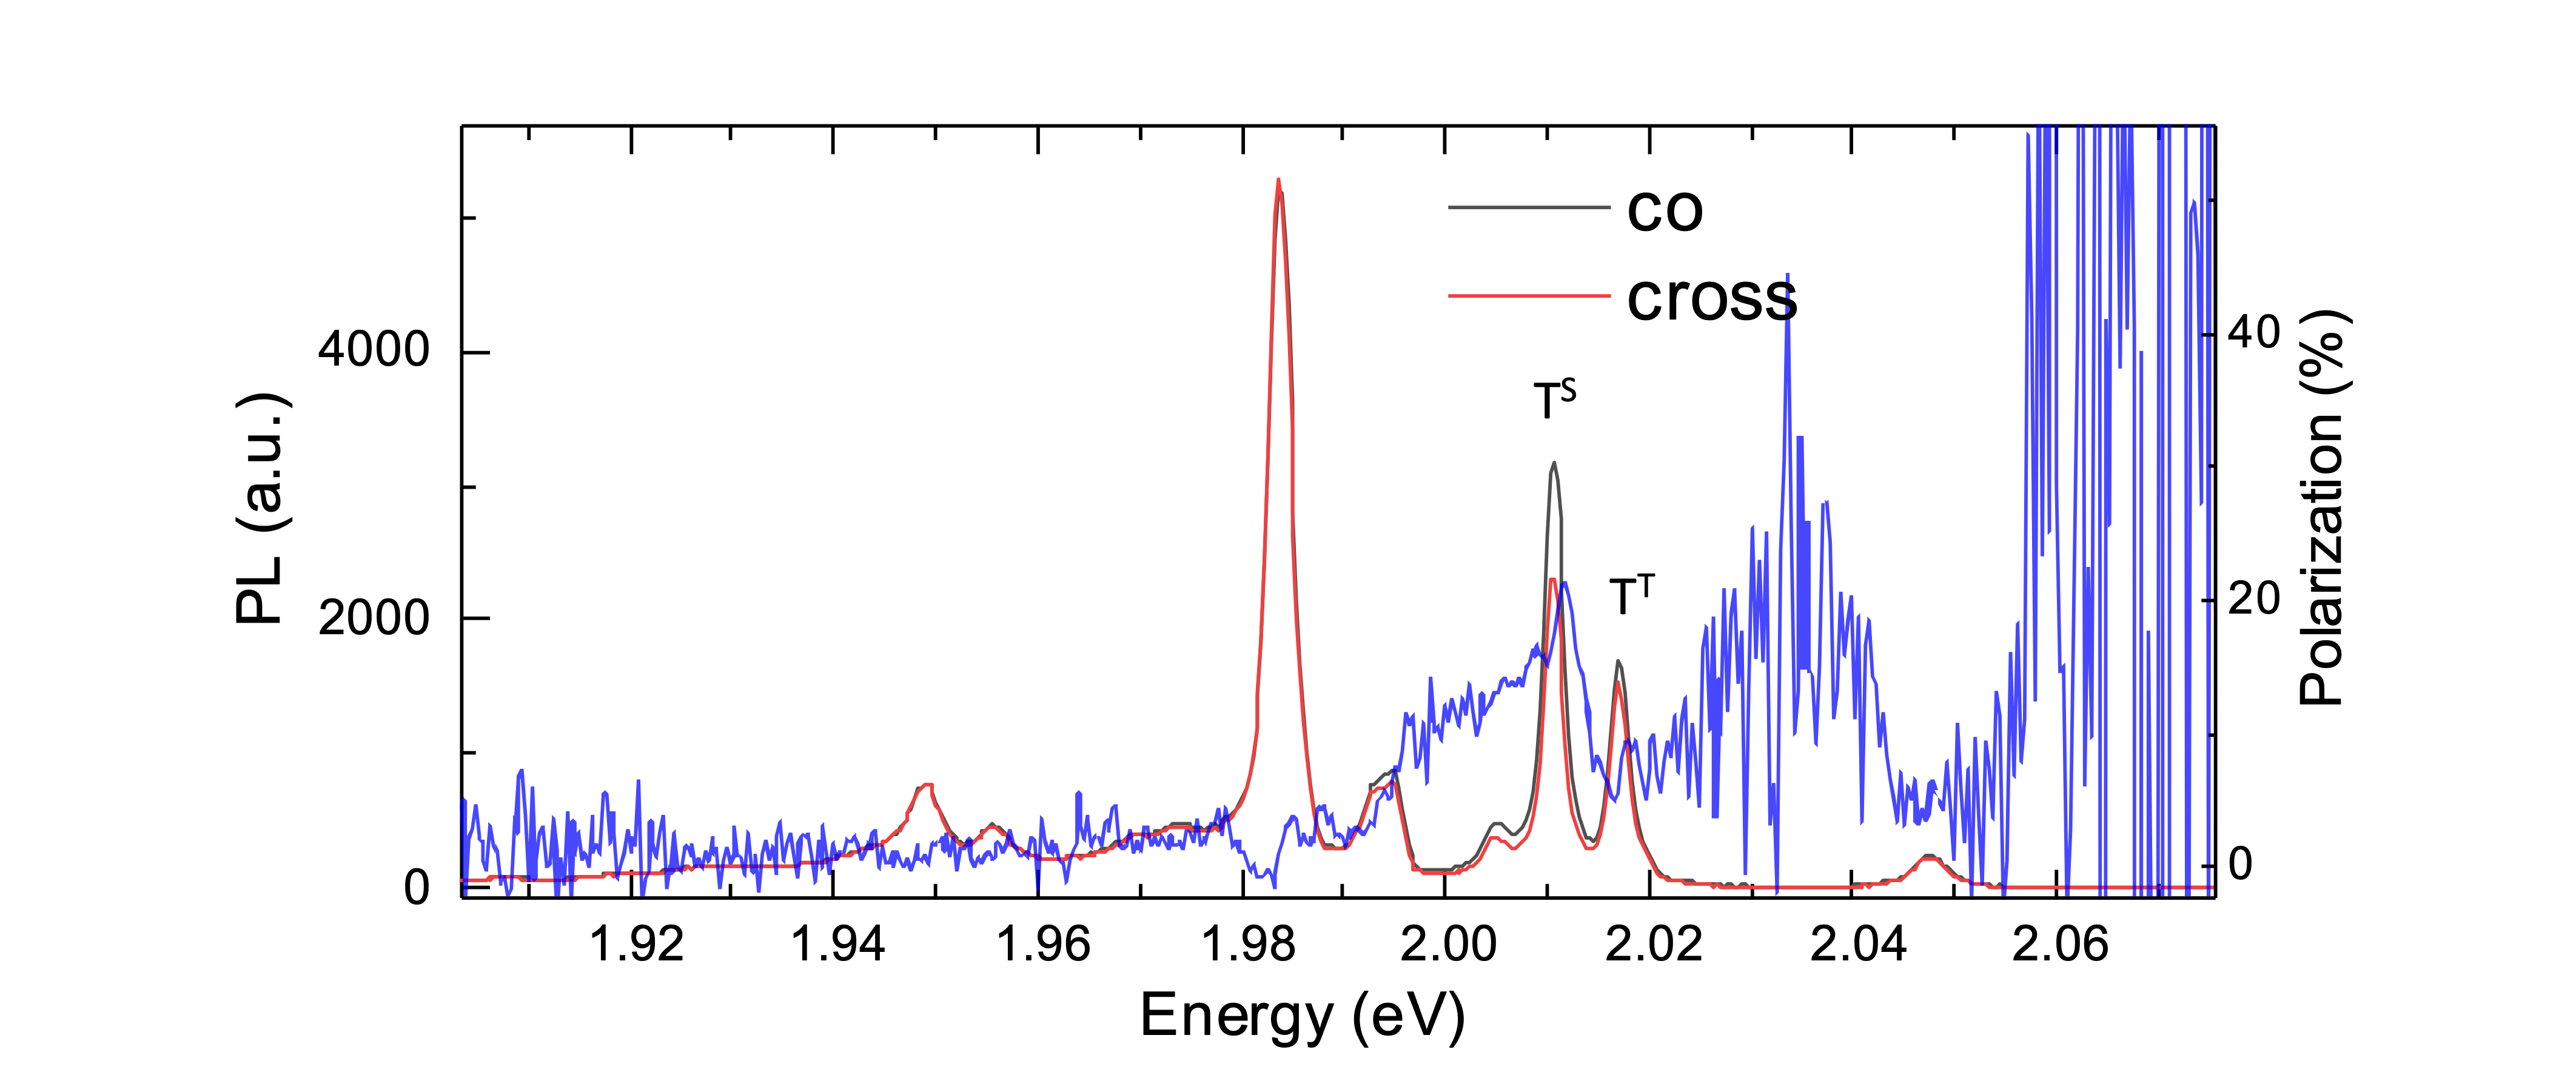
\includegraphics[width=\textwidth]{Figure/Chapter_four/pl_pol_encap.png}
    \caption{Circularly polarized PL spectra of the hBN-encapsulated WS$_2$ monolayer at $T = 3.6$~K. The gray and red lines represent the co-polarized ($\sigma^+/\sigma^+$) and cross-polarized ($\sigma^+/\sigma^-$) spectra, respectively. The lower panel shows the DOCP as a function of photon energy.}
    \label{fig:pl_pol_encap}
\end{figure}

\subsection{PLE Spectroscopy: Exciton and Excited States Resonances}
\label{subsec:PLE Spectroscopy: Exciton and Excited State Resonances}

Photoluminescence excitation (PLE) spectroscopy provides a complementary view of the optical response by mapping the absorption spectrum of the sample. In a PLE measurement, the detection energy is fixed at a chosen emission peak, and the excitation wavelength is scanned; the detected signal as a function of excitation energy traces the absorption resonances that feed the emitting state.

Fig.~\ref{fig:ple_pristine} shows the PLE spectrum of the encapsulated WS$_2$ monolayer, with the detection window centered on the low-energy emission of the sample ($\sim$1.95--2.00~eV region). The excitation was scanned from 450~nm to 610~nm (2.03--2.76~eV) at a power of $P = 4$~$\mu$W. Several distinct resonances are clearly resolved.

The most prominent feature is the A-exciton ground state ($X_A^0$, 1s) at approximately 2.065~eV. The energy of this resonance is $\sim$6~meV higher than the corresponding emission peak in PL, a Stokes shift arising from phonon-assisted relaxation between absorption and emission. At slightly lower energy, the trion resonance $T$ is resolved at $\sim$2.0345~eV, reflecting the binding of a resident electron to the photoexcited exciton.

At $\sim$2.191~eV and $\sim$2.21~eV, the 2s excited states of the trion ($T$:2s) and the neutral A exciton ($X_A^0$:2s) appear as weaker resonances, respectively. The energy spacing of $\sim$145~meV between the $X_A^0$ 1s and 2s states reflects the large exciton binding energy arising from the reduced dielectric screening in the 2D geometry~\cite{chernikov-2014}. At higher energies, the B-exciton resonance $X_B^0$ is observed at $\sim$2.462~eV, corresponding to a valence-band spin--orbit splitting of $\sim$400~meV between the A and B excitons, in good agreement with previously reported values for monolayer WS$_2$~\cite{kormanyos-2015,zhao-2013}.

The PLE spectrum thus provides a complete map of the excitonic absorption hierarchy of the encapsulated WS$_2$ monolayer, confirming the assignment of all spectral features observed in PL and establishing the baseline against which the PLE spectra of annealing-induced emission features will later be compared.

\begin{figure}[htbp]
    \centering
    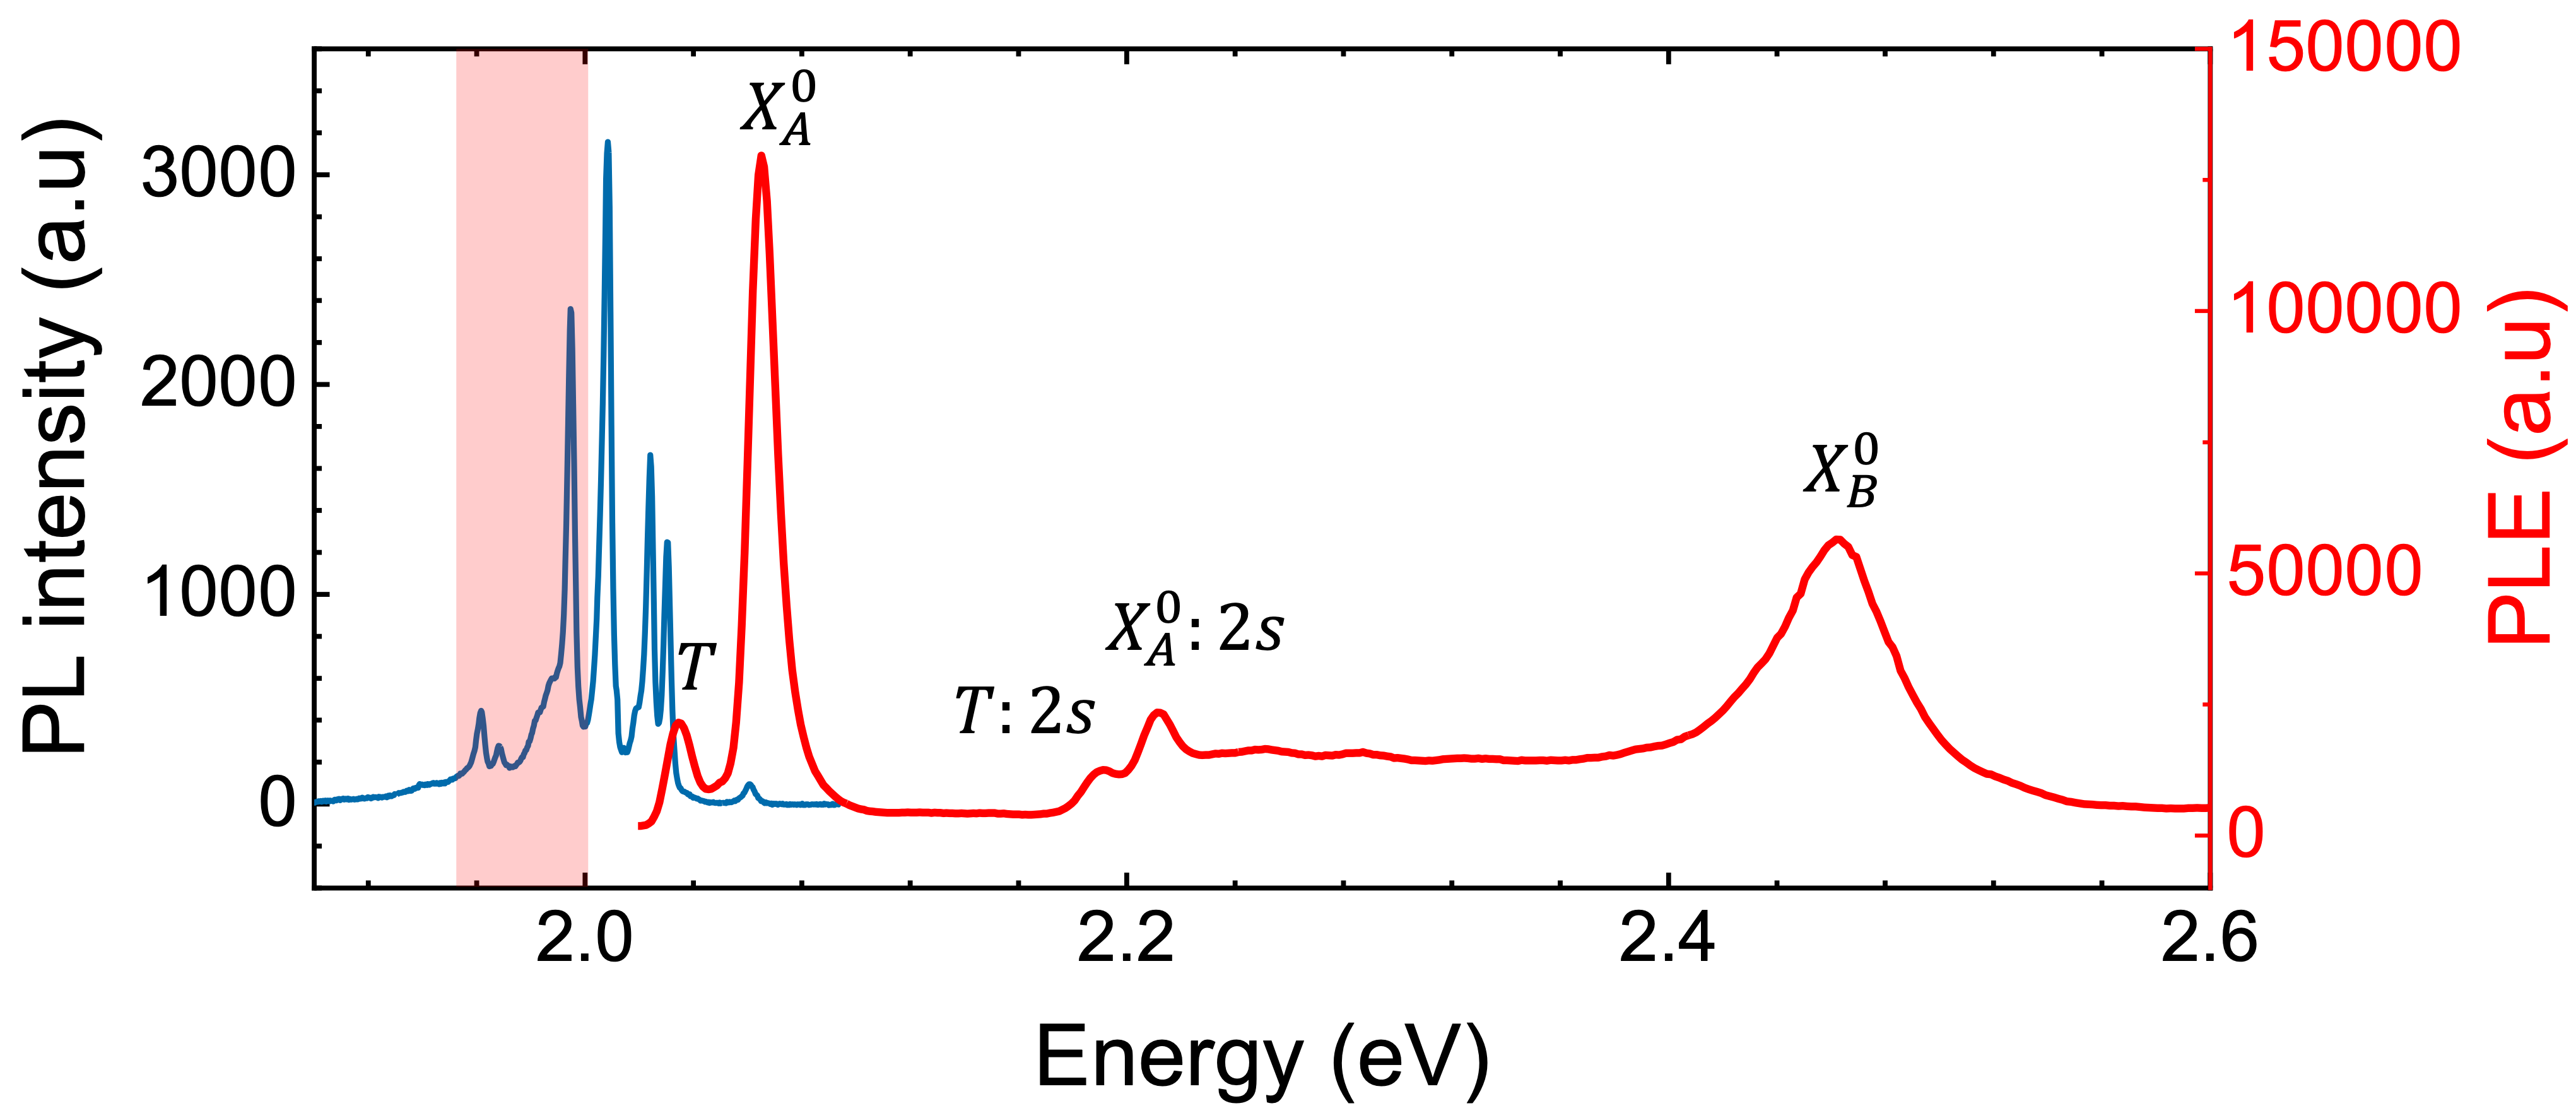
\includegraphics[width=\textwidth]{Figure/Chapter_four/ple_pristine.pdf}
    \caption{PLE spectrum of a pristine hBN-encapsulated WS$_2$ monolayer ($T \approx 4$~K, $P = 1$~$\mu$W), showing resonances at the A-exciton ground state ($X_A^0$: 1s $\approx 2.065$~eV), A-exciton 2s state, trion ($T$), and B exciton ($X_B^0 \approx 2.46$~eV). The inset compares the PLE resonance energy (absorption) with the PL emission energy, illustrating the 6~meV Stokes shift.}
    \label{fig:ple_pristine}
\end{figure}

% \subsection{Optical Quality Comparison with Non-encapsulated Sample}
% \label{subsec:Optical Quality Comparison with Non-encapsulated Sample}


\section{Thermal Activation of Defect Emission in Encapsulated WS$_2$} % (fold)
\label{sec:Thermal Activation}


\subsection{Evolution of Photoluminescence (PL) Spectrum}
\label{subsec:Evolution of PL spectrum}
With the optical baseline established, we now apply the in-situ annealing protocol to the hBN-encapsulated WS$_2$ samples. The annealing temperature is increased step by step from ambient to progressively higher values, with PL spectra recorded after each step at $T_{\mathrm{meas}} \approx 3.6$~K.

Fig.~\ref{fig:pl_encp_annealing} (a) shows the evolution of the PL spectra for a representative encapsulated chip (chip 2-10) across a series of annealing steps. Several distinct stages are observed.

\textbf{Stage I: Spectral stability (up to $\sim$700~K).} Below 700~K, no new spectral features emerge. The excitonic features identified in Section~\ref{subsec:Low-Temperature PL Spectrum}---the neutral exciton, trion doublet, negative biexciton, dark trion $T^I$, semidark trion $T'$, and phonon replicas---are present with unchanged relative energy. 

\textbf{Stage II: Onset of defect emission ($\sim$800~K).} After annealing at 800~K, a new emission peak $X_L'$ appears at $\sim$1.91~eV, situated $\sim$120~meV below the neutral exciton. The peak is spectrally narrow, with a FWHM of a few meV, and constitutes the most intense feature in the spectrum, though the intrinsic excitonic emission remains clearly visible.

\textbf{Stage III: Spectral simplification ($\sim$900~K).} After annealing at 900~K, the intrinsic excitonic emission is markedly suppressed, and the PL spectrum simplifies to a single dominant narrow peak $X_L'$ at $\sim$1.91~eV, as shown in Fig.~\ref{fig:pl_encp_annealing}. The peak is spectrally well-isolated from the remaining excitonic features.

A systematic redshift of all excitonic peaks is observed with increasing annealing temperature, with all relative energy spacings preserved, indicating a rigid ensemble shift of the entire spectrum. Tracking the neutral exciton position $X_A^0$ as a function of annealing temperature reveals a total redshift of $\sim$27.5~meV, from 2.0475~eV after 400~K annealing to 2.020~eV after 900~K annealing.

To enable a direct comparison of the spectral changes induced by annealing, the PL spectra after 400~K and 900~K annealing are replotted with the energy axis referenced to the neutral exciton position $X_A^0$ (\ref{fig:pl_encp_annealing} (b)). This representation eliminates the contribution of the rigid ensemble redshift and allows the intrinsic spectral evolution to be assessed independently. We observe that the intrinsic excitonic peaks are suppressed after 900~K and the new peak $X_L'$ which is at 1.910~eV, corresponding to an energy offset $\Delta E = E(X_A^0) - E(X_L') \approx 120$~meV becomes dominant. This offset is smaller than the $\sim$220~meV offset observed in non-encapsulated samples, possibly related to the well known decrease of binding energy in encapsulated samples due to enhanced dielectric screening \cite{raja-2017}.


\begin{figure}[htbp]
    \centering
    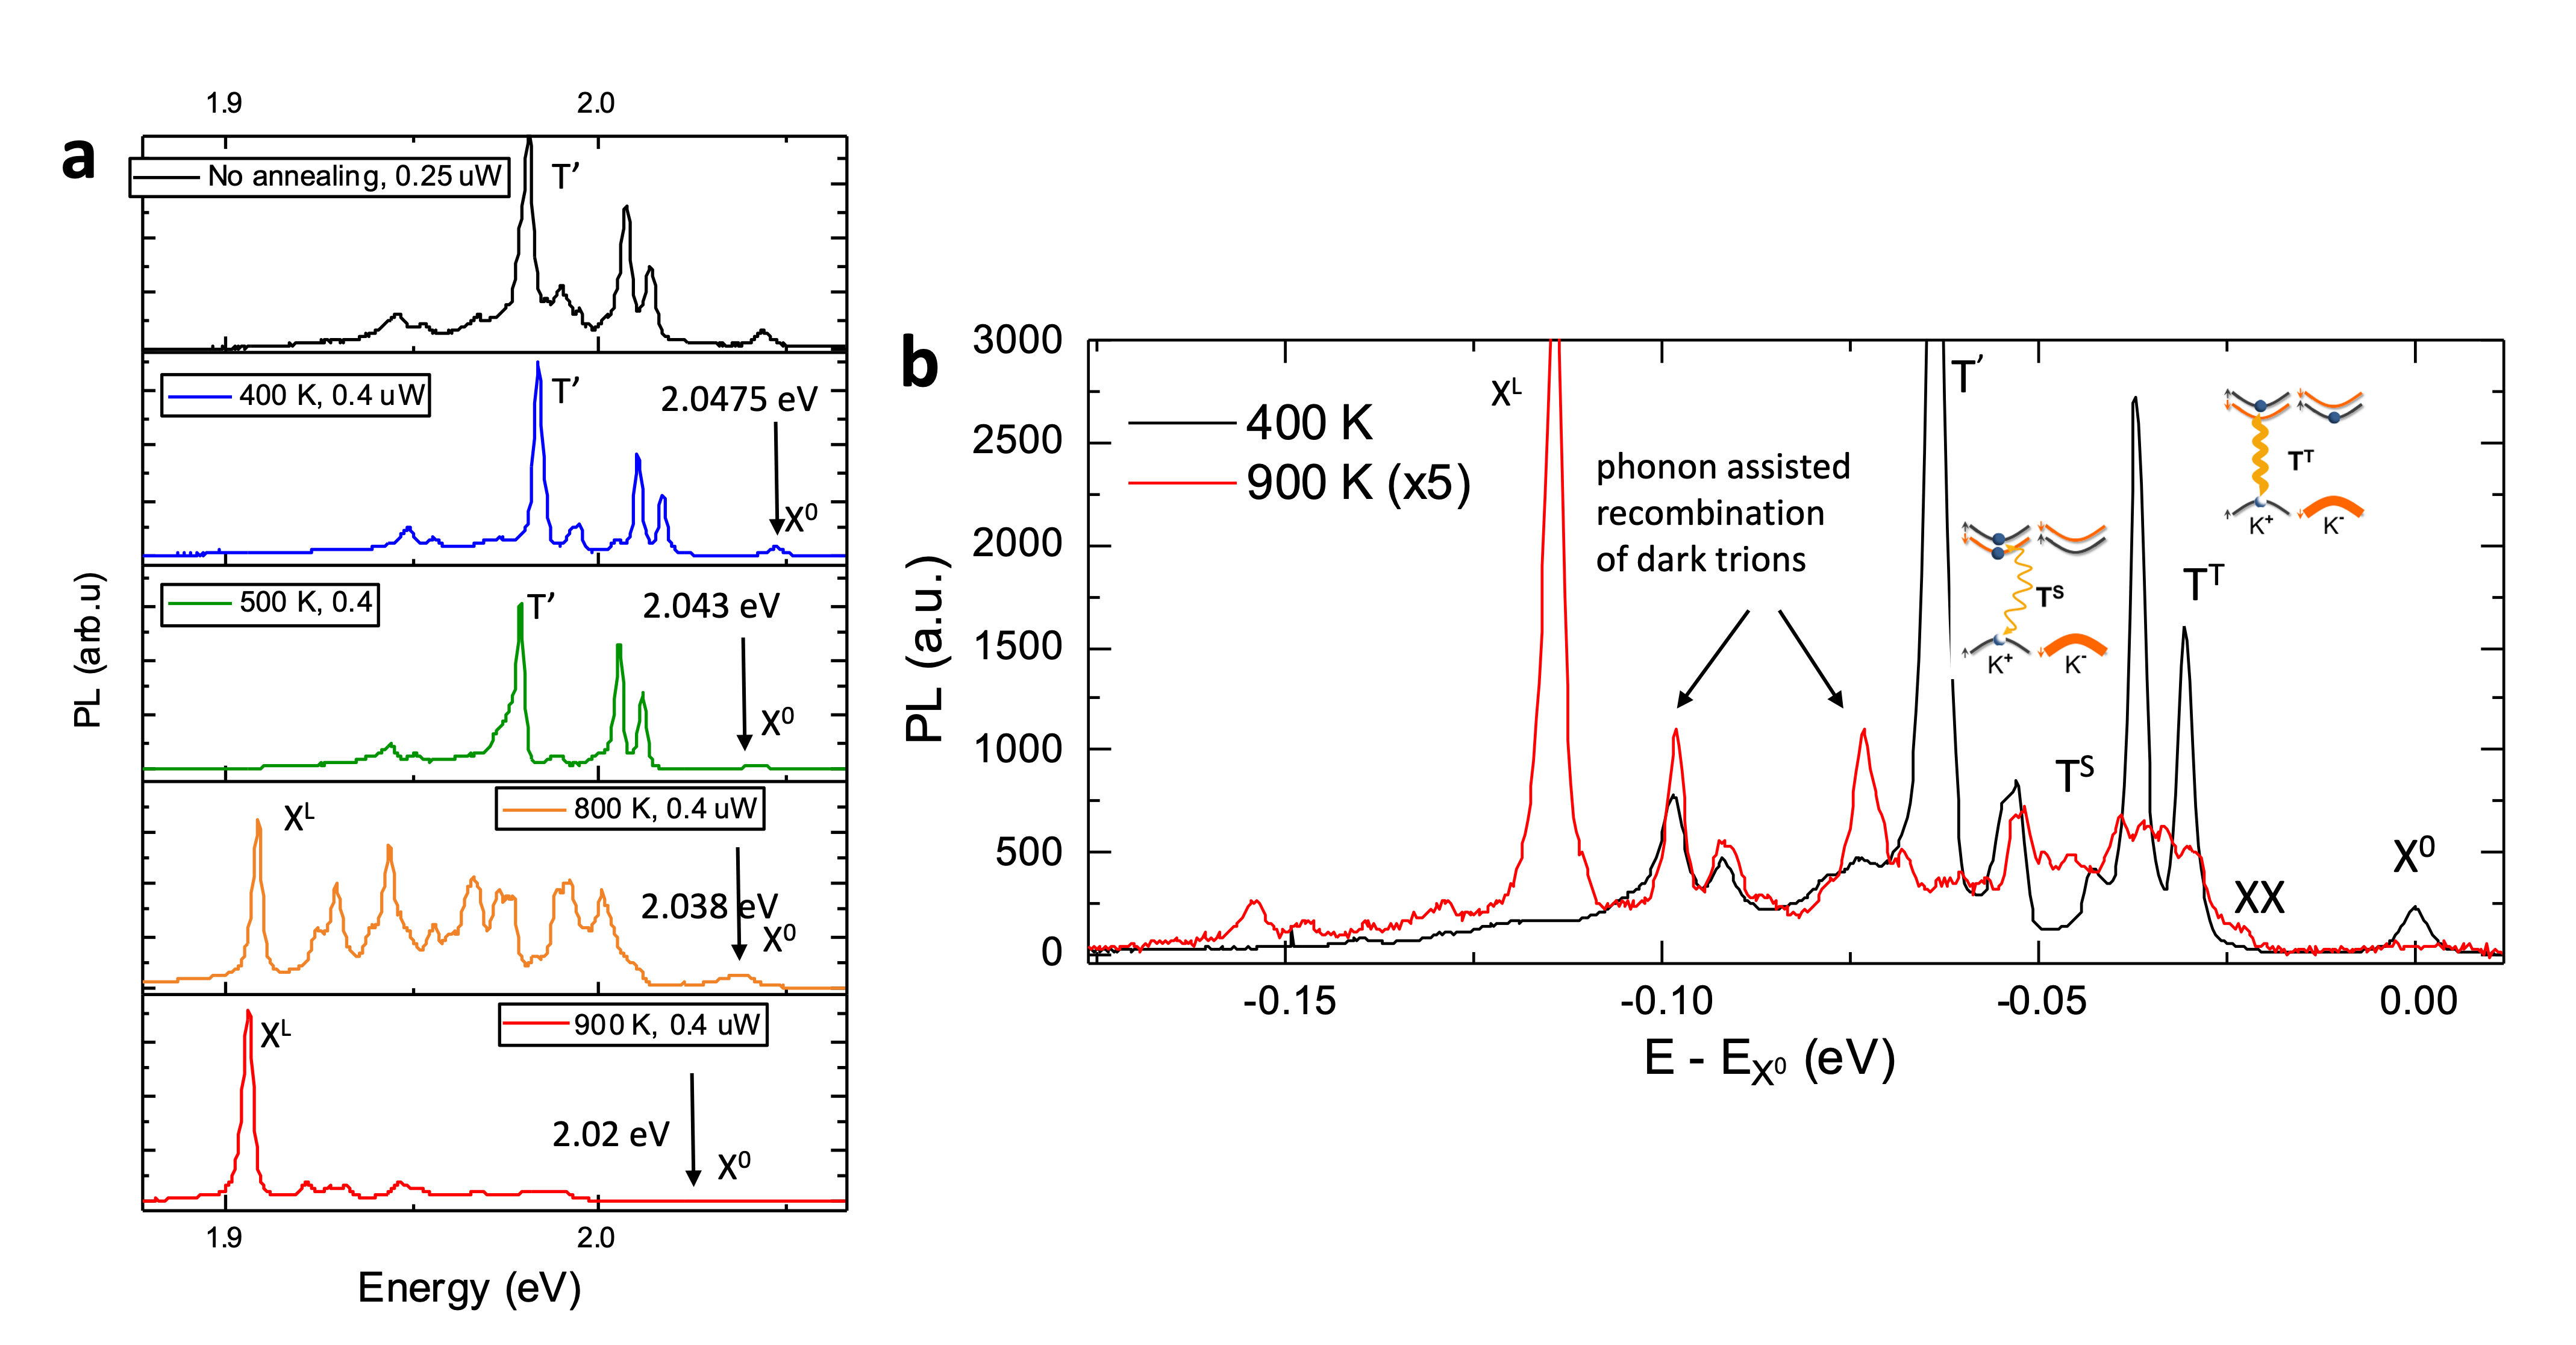
\includegraphics[width=\textwidth]{Figure/Chapter_four/pl_encp_annealing.png}
    \caption{(a) Low-temperature PL spectra of an hBN-encapsulated WS$_2$ monolayer measured at $T = 3.6$~K after annealing at 400, 500, 800, and 900~K for 30~min ($\lambda_{\mathrm{laser}} = 514.5$~nm CW, $P = 0.4$~$\mu$W). (b) Comparison of PL spectra after 400~K and 900~K annealing, with the energy axis referenced to the neutral exciton position $X_A^0$.}
    \label{fig:pl_encp_annealing}
\end{figure}

\subsection{Polarization resolved PL spectrum of $X_L'$}
\label{subsec:Polarization resolved PL spectrum of $X_L'$}

To characterize the polarization properties of $X_L'$, we performed polarization-resolved PL measurements under both circularly and linearly polarized excitation. A pulsed laser at $\lambda = 588$~nm, close to the A-exciton resonance, was used for excitation. Fig.~\ref{fig:pl_xl_prime_pol} shows the resulting spectra under each excitation condition.

Under circularly polarized excitation, the spectrum shows a clear difference between co- and cross-polarized emission, consistent with the valley-selective optical selection rules arising from spin-valley locking at the K and K' points in WS$_2$~\cite{zhu-2015}. In contrast, linearly polarized excitation shows no preferential circular polarization, as expected from the equal population of both valleys. Furthermore, the total PL intensity is noticeably higher under circularly polarized excitation, consistent with efficient spin/valley optical pumping of resident electrons: circular excitation selectively polarizes the resident electrons in one valley, enhancing the formation rate of the bright singlet trion $T^S$ and thereby increasing the overall emission intensity~\cite{robert-2021a}.

\begin{figure}[htbp]
    \centering
    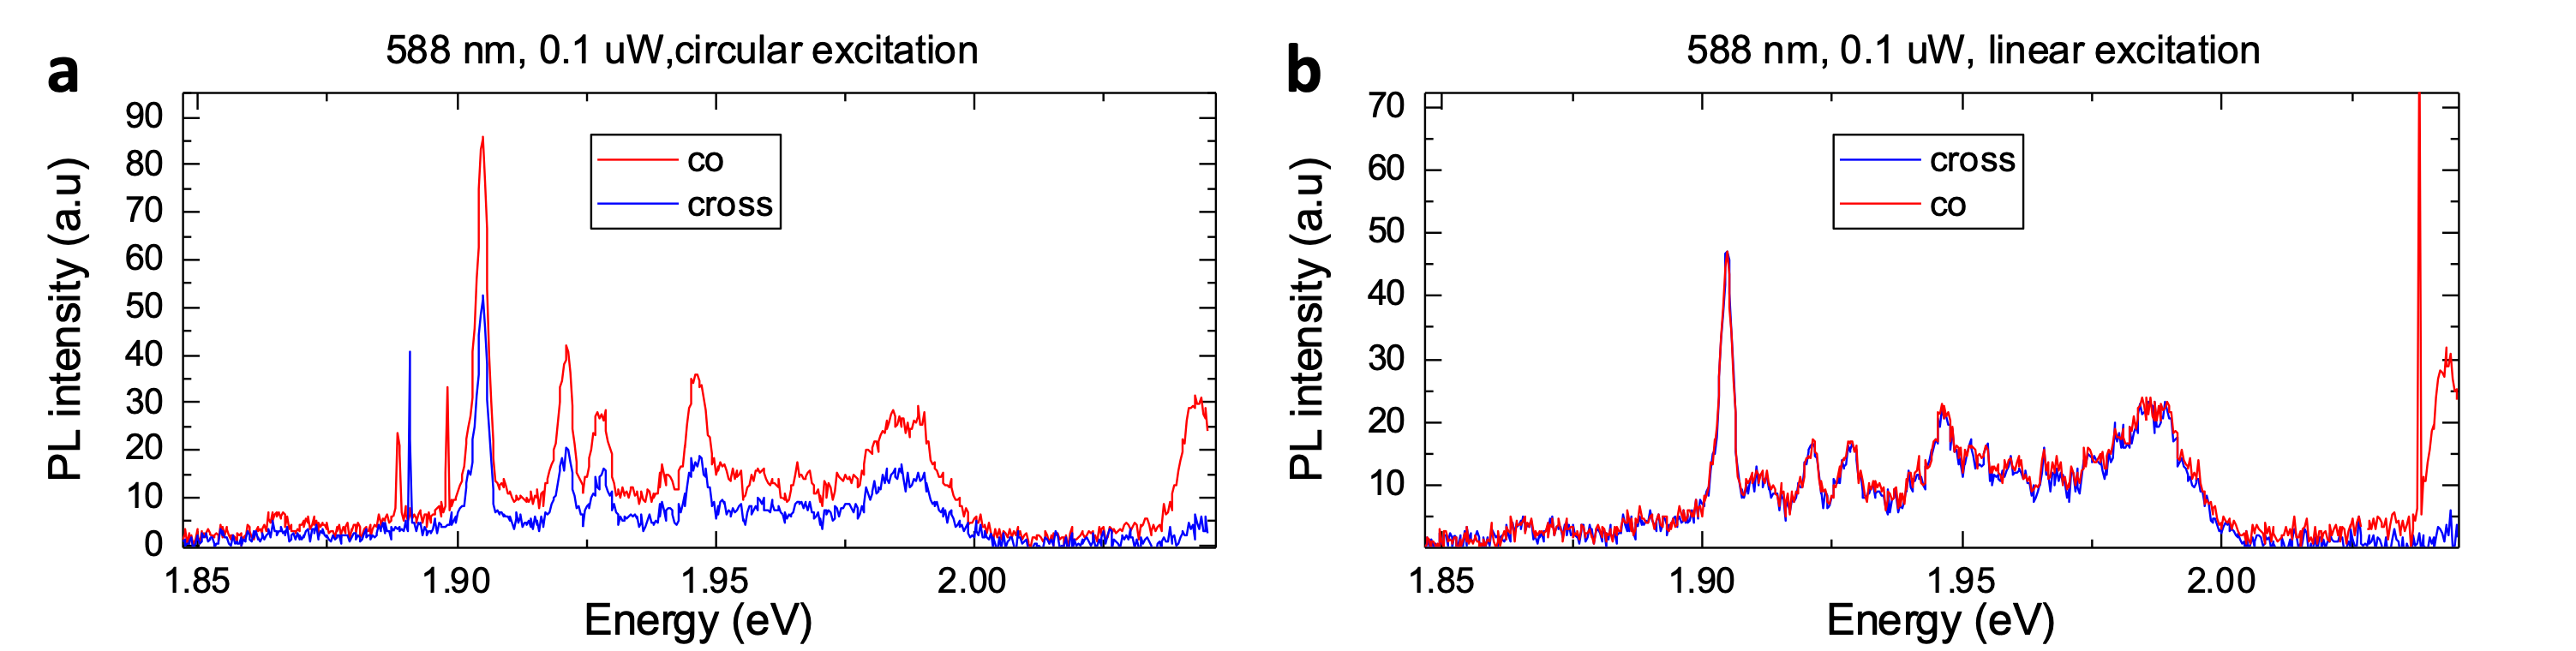
\includegraphics[width=\textwidth]{Figure/Chapter_four/pl_xl_prime_circular_linear.png}
    \caption{Polarization-resolved PL spectra of $X_L'$ after 900~K annealing ($\lambda_{\mathrm{laser}} = 588$~nm, $P = 1~\mu$W, $T = 3.6$~K). (a) Circularly polarized excitation. (b) Linearly polarized excitation.}
    \label{fig:pl_xl_prime_pol}
\end{figure}


\subsection{Power-Dependent Measurements}
\label{subsec:Power-Dependent Measurements}
To characterize the emission behavior of $X_L'$ and confirm its defect-localized nature, we performed power-dependent PL measurements. 

Fig.~\ref{fig:power_dep_pol_encp} shows the power dependence of both the polarization and the emission intensity of $X_L'$ under circularly polarized excitation.
Panels (a) and (b) show the co- and cross-polarized PL spectra at excitation powers of 0.04~$\mu$W and 0.6~$\mu$W, respectively. At the lowest power, $X_L'$ exhibits a pronounced difference between co- and cross-polarized intensities, corresponding to a DOCP exceeding 30\%. As the excitation power increases, this contrast progressively diminishes, and by $\sim$6~$\mu$W the DOCP of $X_L'$ approaches zero, as shown by the right axis of panel (c). This power-induced depolarization is consistent with the generation of free carriers at higher excitation densities, which promotes intervalley scattering and degrades the valley polarization of the defect-localized state.

\begin{figure}[htbp]
    \centering
    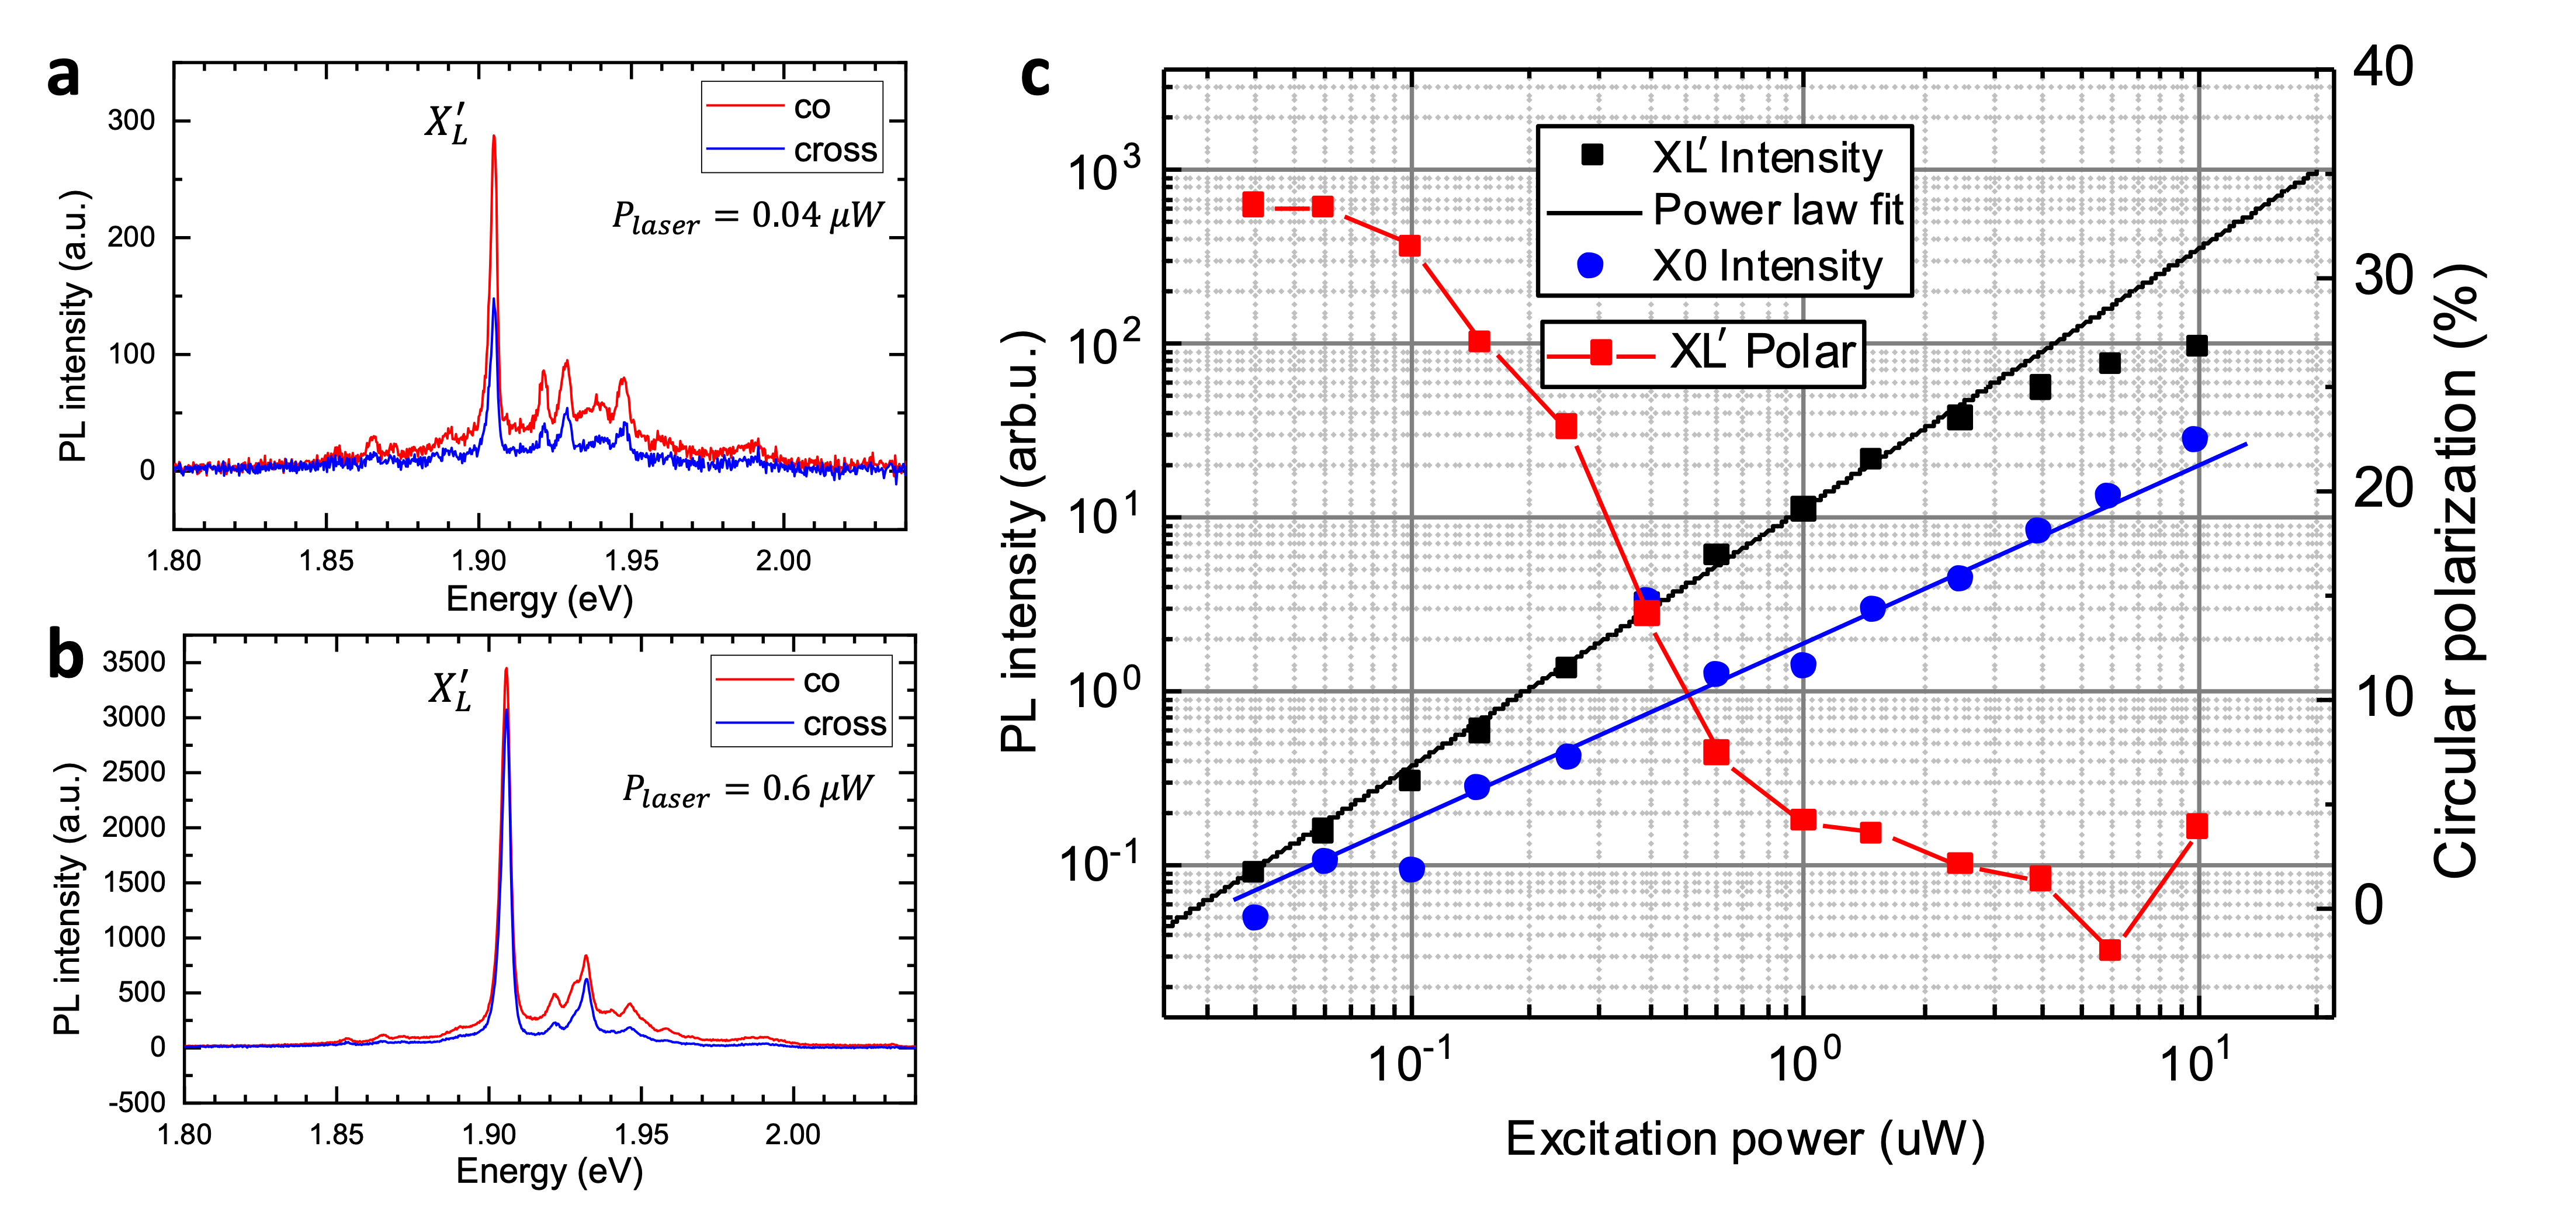
\includegraphics[width=\textwidth]{Figure/Chapter_four/power_dep_pol_encp.png}
    \caption{Power-dependent circularly polarized PL spectra after 900~K annealing ($\lambda_{\mathrm{laser}} = 588$~nm, $T = 3.6$~K). (a) Polarization-resolved PL at $P = 0.04~\mu$W. (b) Polarization-resolved PL at $P = 0.6~\mu$W. (c) Power dependence of the peak intensity of $X_A^0$ and $X_L'$.}
    \label{fig:power_dep_pol_encp}
\end{figure}

Panel (c) also shows the excitation power dependence of the peak intensities of $X_A^0$ (blue) and $X_L'$ (black) on a log--log scale, where the intensities are extracted from Lorentzian fits to each spectrum. The neutral exciton $X_A^0$ exhibits a linear power dependence with a log--log slope of $\sim$1, consistent with a simple single-photon absorption process. In contrast, $X_L'$ shows a super-linear dependence at low excitation powers, with a fitted slope of $\sim$1.5, indicating that the emission dynamics of $X_L'$ are distinct from those of the free exciton and may involve a multi-step excitation pathway. Above $\sim$2.5~$\mu$W, the $X_L'$ intensity deviates from this super-linear regime and begins to saturate, consistent with the finite density of defect states established in Section~\ref{subsec:Power Dependence and Saturation Behavior}. Data above 10~$\mu$W are not shown, as the increasing intensity of surrounding excitonic peaks at high power renders the spectral isolation of $X_L'$ unreliable.


\section{Spectroscopic Origin of Narrow Emission}
\label{sec:Spectroscopic Origin of narrow emission}

The emergence of a defect-related peak $X_L'$ after thermal annealing of encapsulated WS$_2$ raises the fundamental question of its physical origin. Is $X_L'$ intrinsic to WS$_2$, or could it arise from defects or phonon modes in the surrounding hBN layers or the SiC substrate? This section addresses this question using two complementary spectroscopic tools: PLE, which maps the absorption channels feeding the emitting state, and time-resolved PL (TRPL), which probes the lifetime and relaxation dynamics of the excited state.

\subsection{PLE Spectroscopy: Intrinsic WS$_2$ Resonances}
\label{subsec:PLE Spectroscopy: Intrinsic WS$_2$ Resonances}

Fig.~\ref{fig:ple_xl_prime} shows a PLE spectrum recorded with the detection window centered on the $X_L'$ peak energy ($\sim$1.91~eV) at $T = 3.55$~K and $P = 0.25$~$\mu$W, after 900~K annealing of the encapsulated sample.

The PLE spectrum displays a series of well-resolved resonances that can be directly assigned to intrinsic optical transitions of monolayer WS$_2$. The dominant resonances appear at approximately 2.025~eV ($X_A^0$: 1s) and 1.99~eV (trion $T$), along with their respective 2s excited states. This pattern is consistent with the PLE spectrum of the pristine encapsulated sample (Section~\ref{subsec:PLE Spectroscopy: Exciton and Excited State Resonances}), confirming that $X_L'$ is activated by the same optical transitions as the intrinsic excitonic emission.

\begin{figure}[htbp]
    \centering
    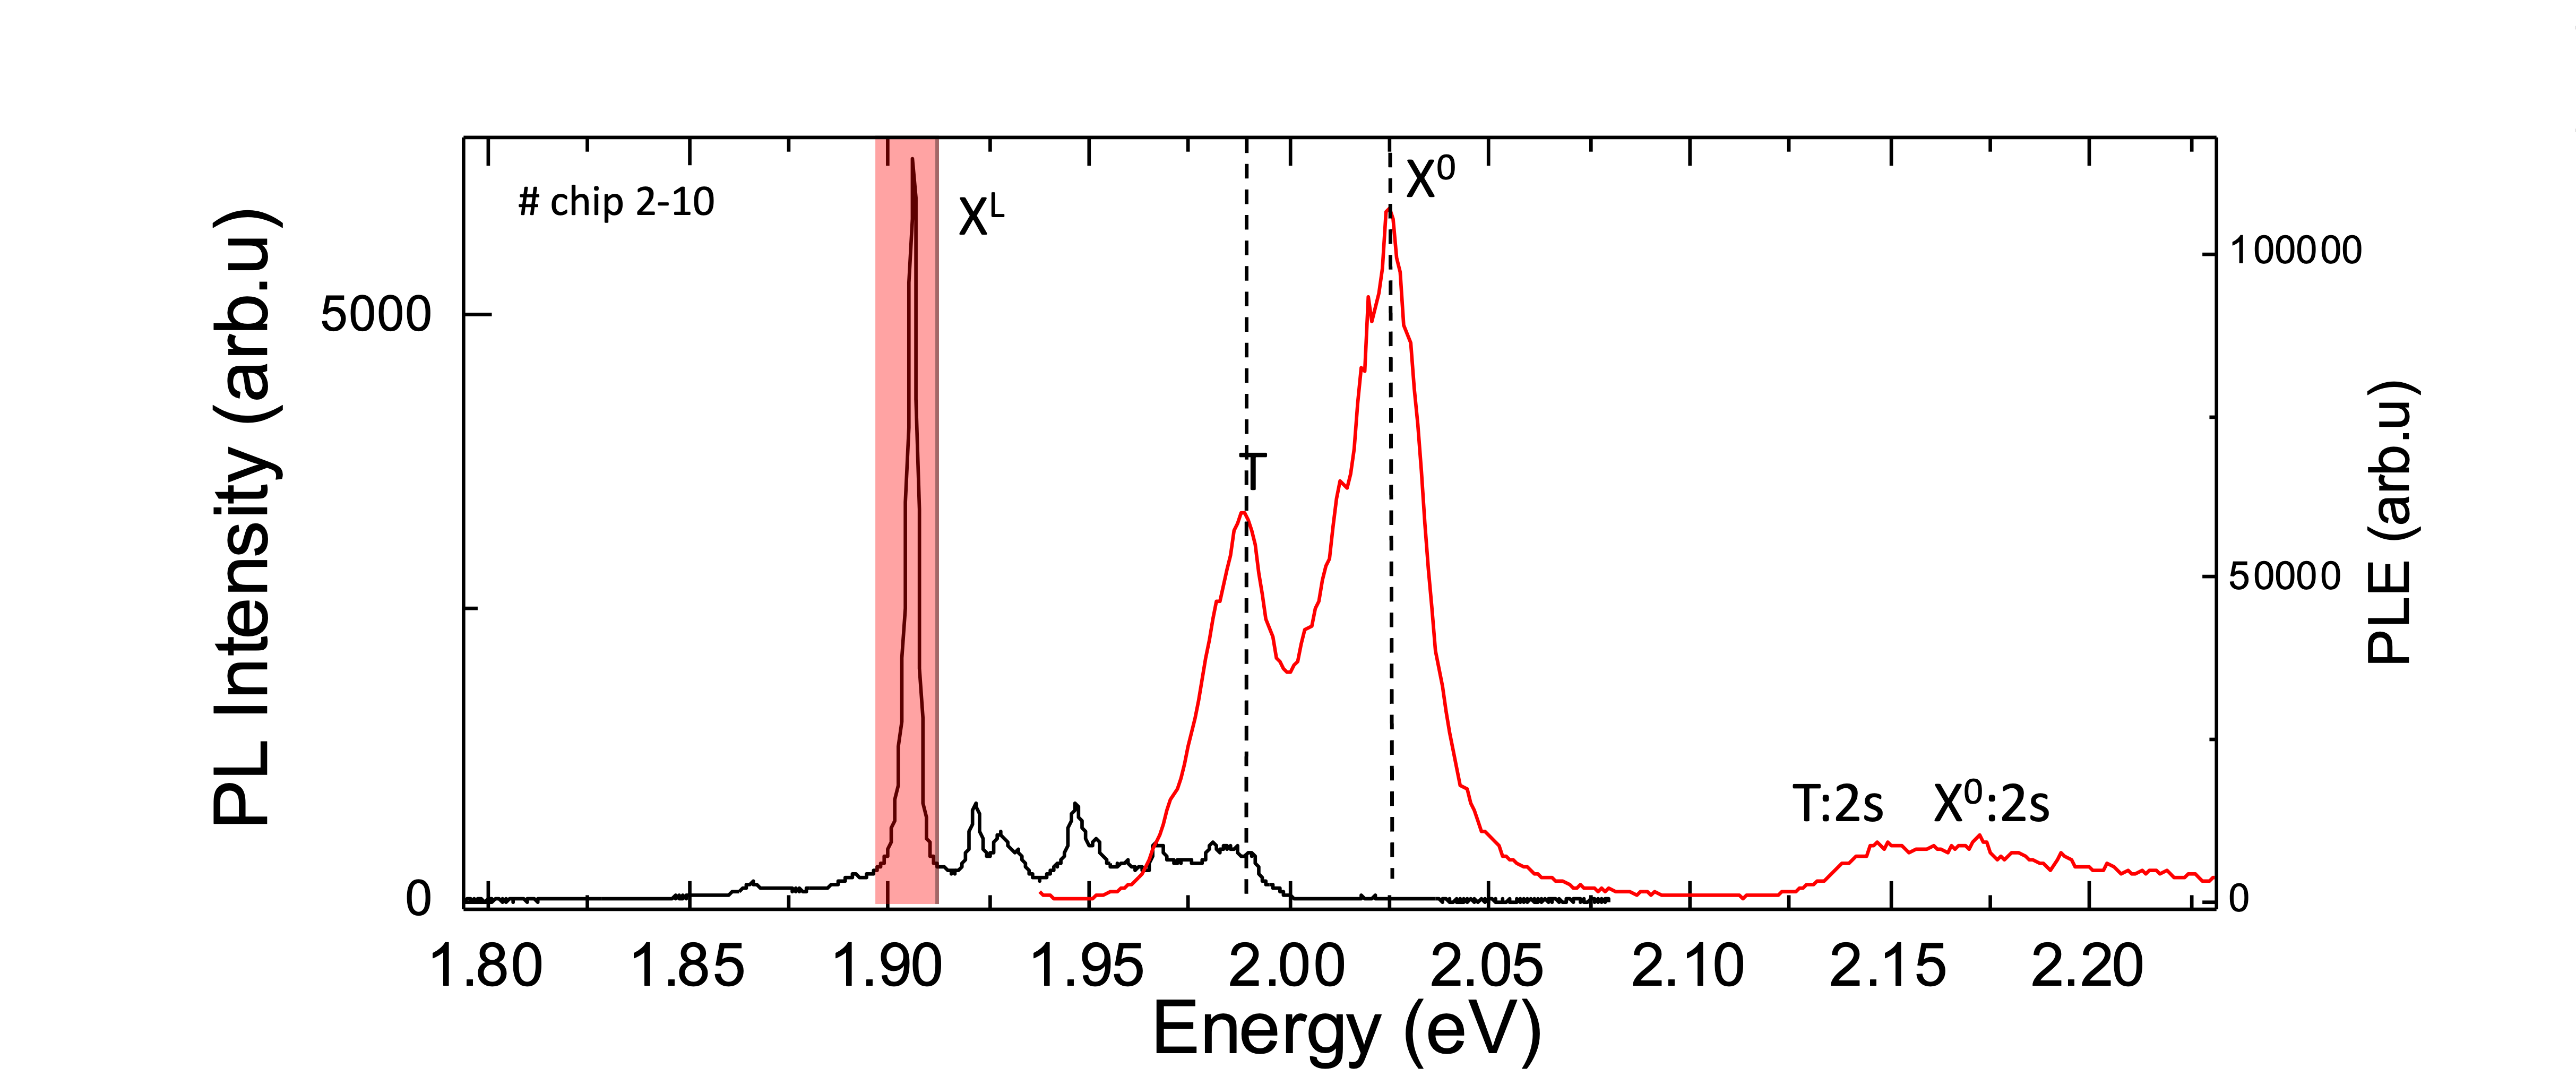
\includegraphics[width=\textwidth]{Figure/Chapter_four/ple_xl_prime.png}
    \caption{PLE spectrum of the $X_L'$ emission in the encapsulated WS$_2$ sample after 900~K annealing ($T = 3.55$~K, $P = 0.25$~$\mu$W, detection at $\sim$1.91~eV). Resonances at the A exciton ($X_A^0$: 1s), trion ($T$), and their 2s excited states are resolved, confirming the intrinsic WS$_2$ origin of $X_L'$. The energy offset between the $X_A^0$ absorption and the $X_L'$ emission is $\sim$120~meV.}
    \label{fig:ple_xl_prime}
\end{figure}

These PLE resonances indicate that $X_L'$ is populated via absorption in the WS$_2$ host lattice: free excitons generated at the A-exciton or trion resonances diffuse through the monolayer and become localized at defect sites, rather than being excited by direct absorption into the defect state itself. 

The Stokes shift between the PLE resonance at the A-exciton energy and the $X_L'$ emission peak is approximately 120~meV. This large Stokes shift is the defining signature of exciton localization: it measures the energy difference between the free A-exciton and the localized defect state, indicating that the defect potential well binds the exciton with significant localization energy.


\subsection{Time-Resolved PL: Radiative Lifetime and Decay Dynamics}
\label{subsec:Time-Resolved PL: Radiative Lifetime and Decay Dynamics}

Time-resolved photoluminescence (TRPL) provides direct access to the lifetime of $X_L'$ and its decay dynamics. The measurements were performed using a pulsed laser with a 40~ps pulse width and repetition rate of 78~MHz, with emitted photons detected by a single-photon avalanche diode (SPAD) coupled to a two-stage spectrometer. The temporal resolution of the TCSPC system is approximately 40~ps.

Fig.~\ref{fig:trpl_xl_prime}(a) shows a two-dimensional time-energy map acquired on chip 2-10 at $T = 3.51$~K ($\lambda_{\mathrm{laser}} = 578$~nm, $P = 0.6$~$\mu$W), plotting photon arrival time relative to the laser pulse on the vertical axis and emission energy on the horizontal axis. The time-averaged PL spectrum in Fig.~\ref{fig:trpl_xl_prime}(b) confirms that $X_L'$ is the dominant emission feature in this energy window.

Fig.~\ref{fig:trpl_xl_prime}(c) shows the decay curves extracted for the bright trion, the phonon-assisted dark trion peaks $T_{D3}$ and $T_{D4}$, and $X_L'$. The bright-exciton and trion emissions rise promptly after the laser pulse and decay rapidly with characteristic times of $\lesssim 100$~ps, consistent with the fast radiative recombination of bright excitons in WS$_2$. The phonon-assisted dark trion peaks $T_{D3}$ and $T_{D4}$ exhibit a notably longer lifetime of $\sim$700~ps, reflecting the indirect nature of their recombination pathway: zone-edge phonons are required to provide the momentum and spin conservation necessary for radiative recombination, which reduces the effective oscillator strength and extends the lifetime, consistent with the long-lived character of dark trion states in WS$_2$~\cite{zinkiewicz-2020a}.

The $X_L'$ emission region displays a clearly delayed onset of approximately 200~ps relative to the other excitonic features, indicating that free excitons generated by the laser must first diffuse to and be captured by the defect sites before $X_L'$ emission can occur. After this delayed rise, the decay follows a single-exponential function $I(t) \propto \exp(-t/\tau)$ with a fitted lifetime of $\tau \approx 513$~ps. These results confirm that $X_L'$ corresponds to a well-defined radiative recombination channel, clearly distinct from the intrinsic excitonic features of WS$_2$.

\begin{figure}[htbp]
    \centering
    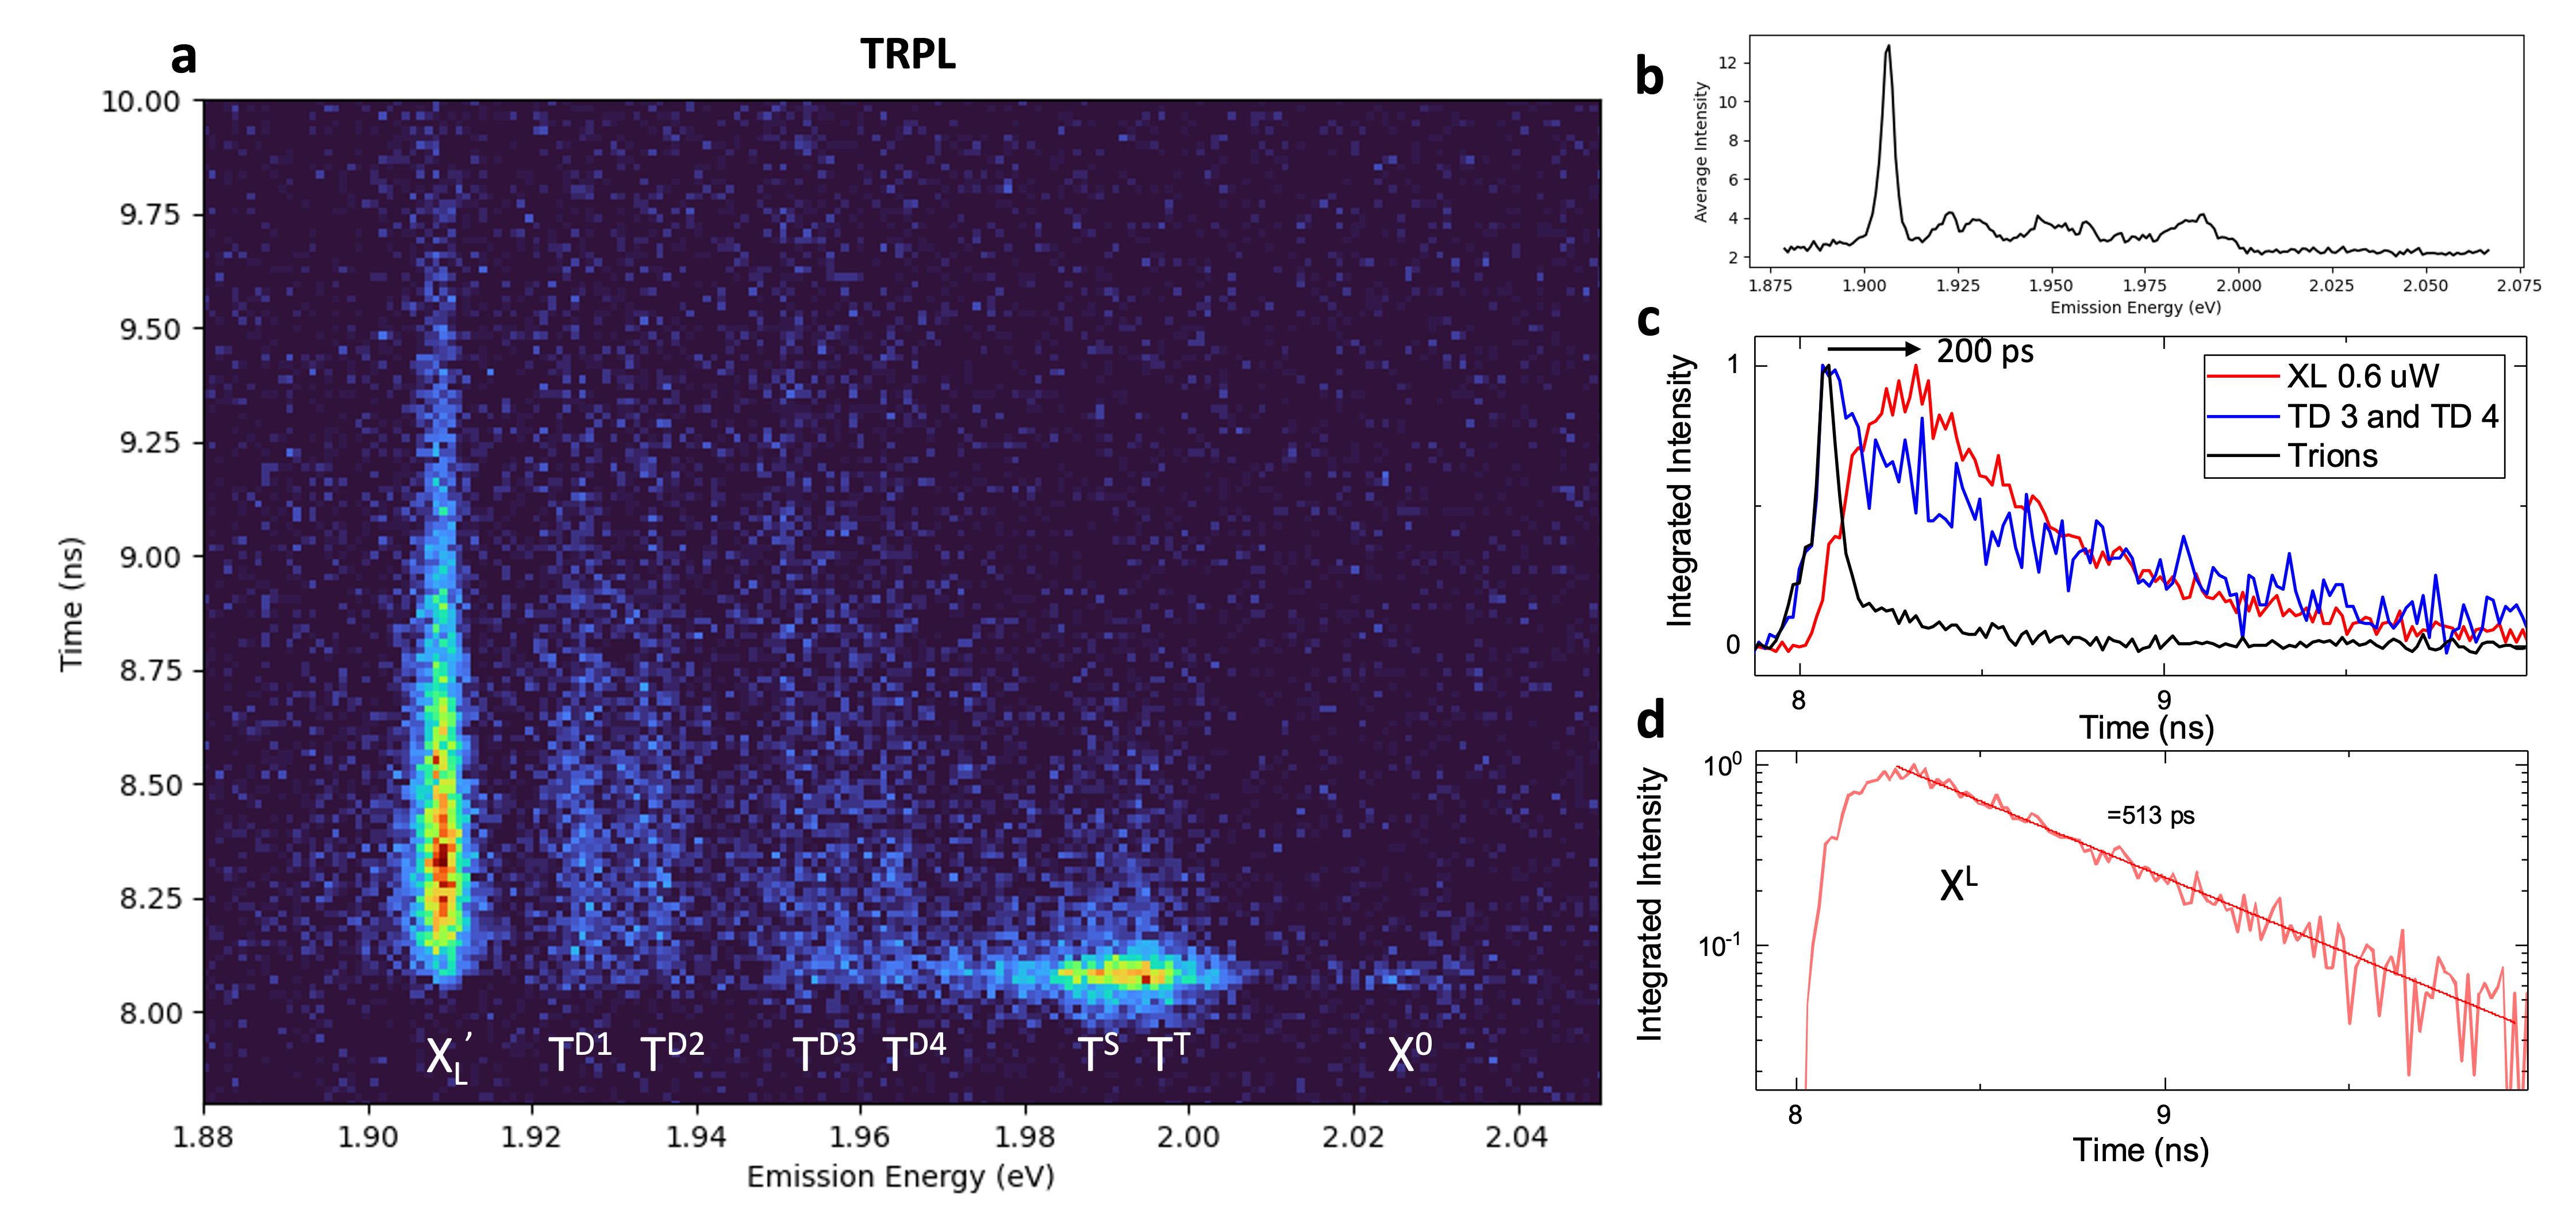
\includegraphics[width=\textwidth]{Figure/Chapter_four/trpl_xl_prime.png}
    \caption{(a) TRPL time--energy map of the encapsulated WS$_2$ sample (chip 2-10) at $T = 3.51$~K ($\lambda_{\mathrm{laser}} = 578$~nm, $P = 0.6$~$\mu$W). (b) Time-averaged PL spectrum extracted from the map, showing $X_L'$ as the dominant feature. (c) Decay curves of the bright trion, phonon-assisted dark trion peaks $T_{D3}$ and $T_{D4}$, and $X_L'$ on a semi-logarithmic scale. The $X_L'$ onset is delayed by $\sim$200~ps; the single-exponential fit yields $\tau \approx 513$~ps.}
    \label{fig:trpl_xl_prime}
\end{figure}

\section{Conclusion}

In this chapter, we have presented a systematic spectroscopic investigation of thermally activated defect emission in WS$_2$ monolayers, from the initial observation in non-encapsulated samples to the detailed characterization of a well-defined defect emitter in hBN-encapsulated heterostructures. In non-encapsulated WS$_2$, high-temperature annealing above $\sim$1000~K activates a broad localized emission $X_L$ at $\sim$220~meV below the neutral exciton, exhibiting saturation behavior consistent with a finite density of defect states and thermal quenching above $\sim$100~K. These limitations motivated the transition to hBN-encapsulated samples, which not only dramatically improved the optical quality of the sample but also provided a well-resolved excitonic baseline---including the neutral exciton, trion doublet, dark excitonic complexes, and their phonon replicas---against which annealing-induced spectral changes could be unambiguously identified.

In encapsulated WS$_2$, a spectrally narrow emission $X_L'$ appears already at 800~K annealing and becomes the dominant spectral feature after 900~K. The emission at $\sim$1.91~eV, located $\sim$120~meV below $X_A^0$, exhibits super-linear power dependence with saturation at a finite excitation density, a high degree of circular polarization at low power, and PLE resonances exclusively at intrinsic WS$_2$ transitions, confirming its localized defect nature and WS$_2$ origin. TRPL measurements reveal a delayed onset of $\sim$200~ps and a single-exponential decay with lifetime $\tau \approx 513$~ps, clearly distinct from the fast dynamics of intrinsic excitonic features. Taken together, these results establish $X_L'$ as a well-defined radiative recombination channel associated with thermally induced defects in WS$_2$. The quantum optical nature of this emission---specifically, whether $X_L'$ operates as a single-photon emitter---is addressed in Chapter~\ref{chap:five}.









% section second_section (end)


% ---- bibliography

% \printbibliography[heading=subbibintoc]  % 잠시 주석처리


% \bibliographystyle{apalike}
% \bibliography{bib_thesis}


\end{document}
